%% Bookheader, Nov 8, 2020; July 18, 2022

\documentclass[11pt]{../Support/ourbook}
%% or for landscape, comment out line above and use this one:
%%\documentclass[landscape,11pt]{ourbook}

%% This will keep space from stretching around display math:

\makeatletter
\renewcommand\normalsize{%
   \@setfontsize\normalsize\@xipt{13.6}%
   \abovedisplayskip 11\p@  \@minus6\p@
   \abovedisplayshortskip \z@ 
   \belowdisplayshortskip 6.5\p@ \@minus3\p@
   \belowdisplayskip \abovedisplayskip
   \let\@listi\@listI}
\makeatother
\normalsize


\begin{document}

\tableofcontents
\graphicspath{{../../Chapters/sound/en_US}}
\chapter{Sound}

When you set off a firecracker, it makes a sound.

Let's break that down a little more. Inside the cardboard wrapper of
the firecracker, there is potassium nitrate ($KNO_3$), sulfur ($S$),
and carbon($C$).  These are all solids. When you trigger the chemical
reactions with a little heat, these atoms rearrange themselves to be
potassium carbonate ($K_2CO_3$), potassium sulfate ($K_2SO_4$), carbon
dioxide ($CO_2$), and nitrogen ($N_2$). Note that the last two are
gasses.

The molecules of a solid are much more tightly packed than the
molecules of a gas. So after the chemical reaction, the molecules
expand to fill a much bigger volume. The air molecules nearby get
pushed away from the firecracker.  They compress the molecules beyond
them, and those compress the molecules beyond them.

This compression wave radiates out as a sphere; its radius growing at
about 343 meters per second (``The speed of sound'').

The energy of the explosion is distributed around the surface of this
sphere. As the radius increases, the energy is spread more and more
thinly around. This is why the firecracker seems louder when you are
closer to it. (If you set off a firecracker in a sewer pipe, the sound
will travel much, much farther.)

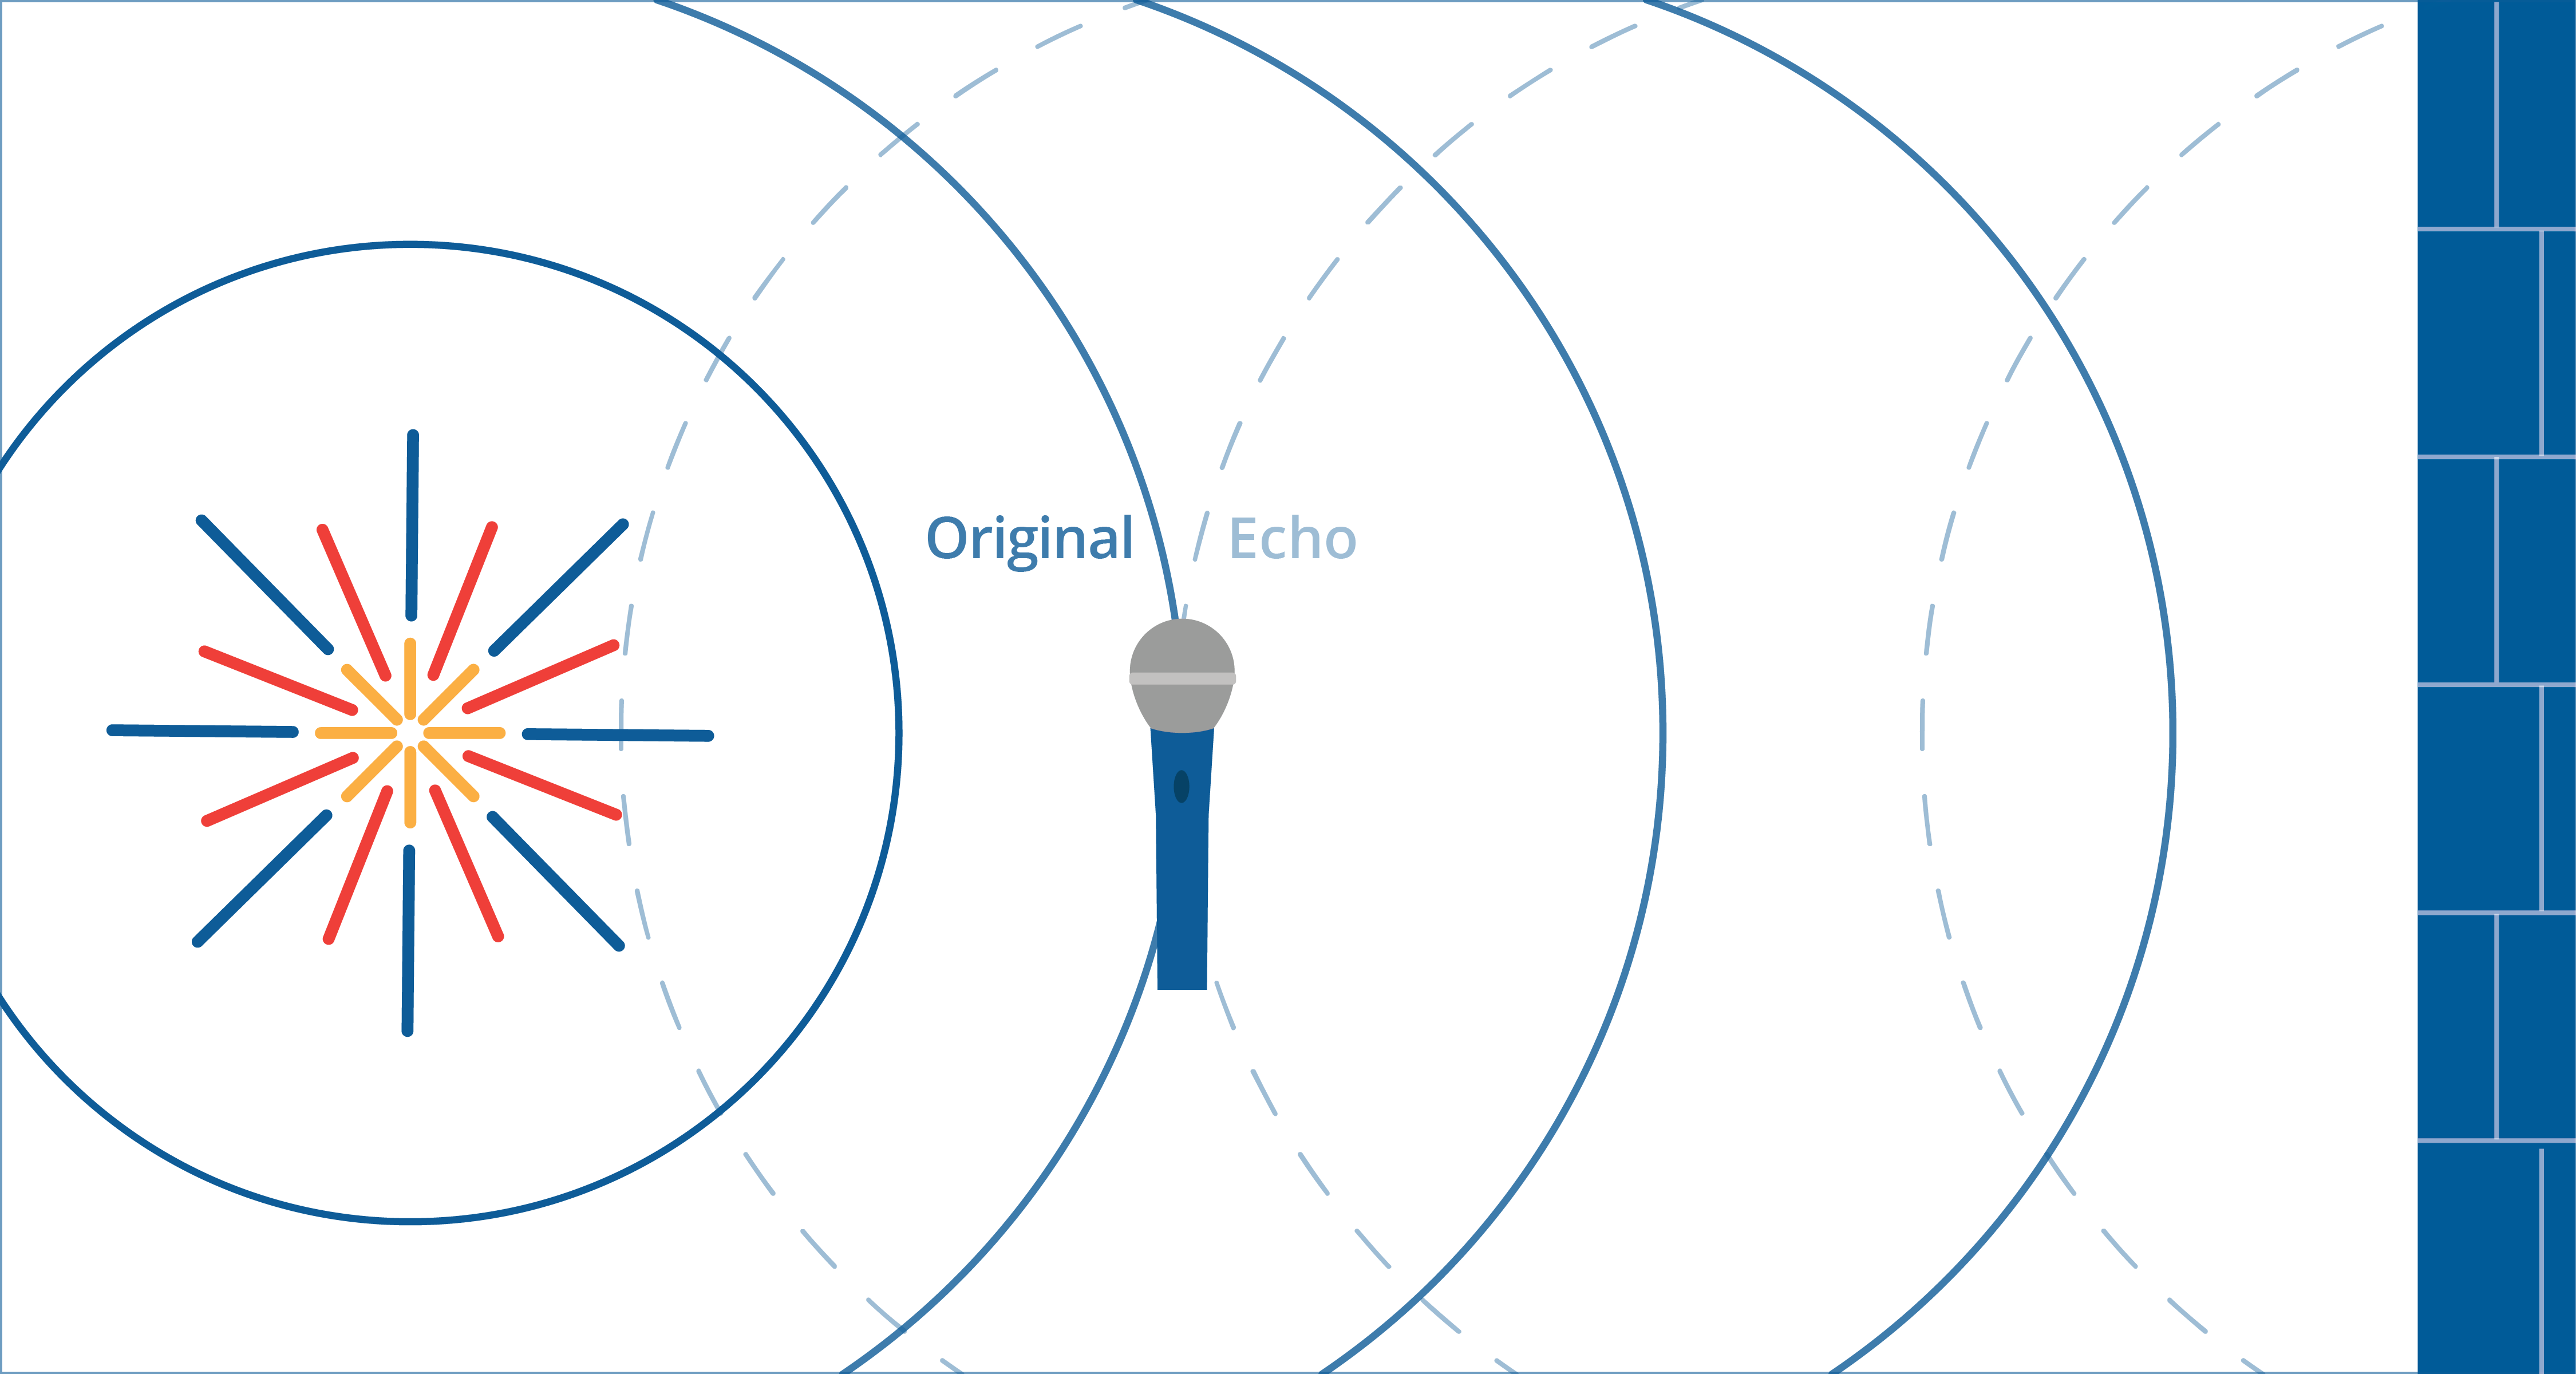
\includegraphics[width=1\textwidth]{firecracker.png}


This compression wave will bounce off of hard surfaces. If you set off
a firecracker 50 meters from a big wall, you will hear the explosion
twice. We call the second one an ``echo''.

The compression wave will be absorbed by soft surfaces. If you covered
that wall with pillows, there would be almost no echo.

The study of how these compression waves move and bounce is called
\newterm{acoustics}. Before you build a concert hall, you hire an
acoustician to look at your plans and tell you how to make it sound
better.

\section{Pitch and frequency}

The string on a guitar is very similar to the weighted spring
example. The farther the string is displaced, the more force it feels
pushing it back to equilibrium. Thus, it moves back and forth in a
sine wave. (OK, it isn't a pure sine wave, but we will get to that later.)

The string is connected to the center of the boxy part of the guitar,
which is pushed and pulled by the string. That creates compression
waves in the air around it.

If you are in the room with the guitar, those compression waves enter
your ear and push and pull your eardrum, which is attached to bones that
move a fluid that tickles tiny hairs, called \newterm{cilia}, in your
inner ear. This is how you hear.

We sometimes see plots of sound waveforms.  The $x$-axis represents
time. The $y$-axis represents the amount the air is compressed at the
microphone that converted the air pressure into an electrical signal.

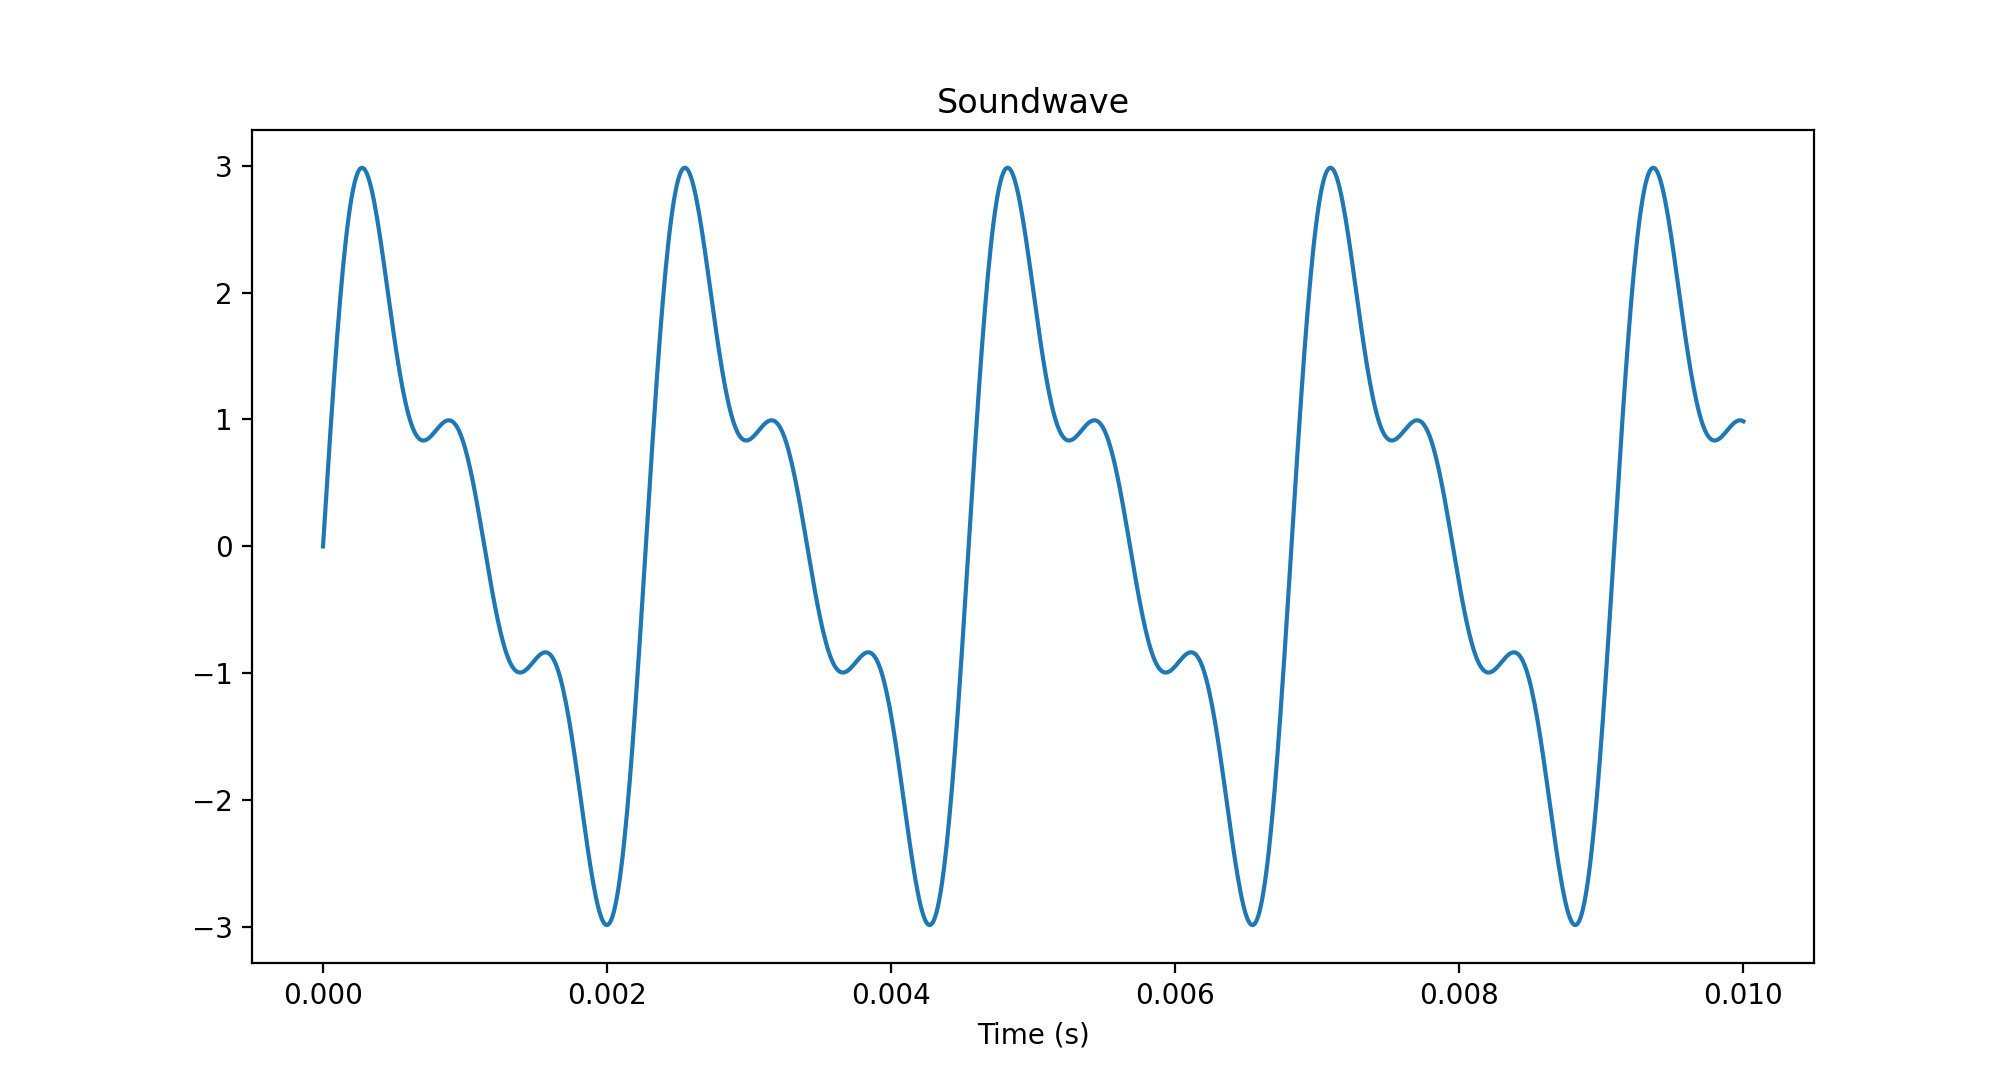
\includegraphics[width=0.8\linewidth]{soundwave.png}

If the guitar string is made tighter (by the tuning pegs) or shorter
(by the guitarist's fingers on the strings), the string vibrates more
times per second.  We measure the number of waves per second and we
call it the \newterm{frequency} of the tone. The unit for frequency is
\newterm{Hertz}: cycles per second.

Musicians have given the different frequencies names. If the guitarist
plucks the lowest note on his guitar, it will vibrate at 82.4
Hertz. The guitarist will say ``That pitch is low E.'' If the string is made
half as long (by a finger on the 12th fret), the frequency will be
twice as fast (164.8 Hertz), and the guitarist will say ``That is E an
octave up.''

For any note, the note that has twice the frequency is one octave
up. The note that has half the frequency is one octave down.

The octave is a very big jump in pitch, so musicians break it up into
12 smaller steps. If the guitarist shortens the E string by one fret,
the frequency will be $82.4 \times 1.059463 \approx 87.3$ Hertz. 

Shortening the string one fret always increases the frequency by a factor of 1.059463. Why?

Because $1.059463^12 = 2$. That is, if you take 12 of these hops, you
end up an octave higher.

This, the smallest hop in western music, is referred to as a \newterm{half step}.

\begin{Exercise}[title={Notes and frequencies}, label=note_to_frequency]

The note A near the middle of the piano, is 440Hz. The note E is 7 half steps above A.  What is its frequency?
 
\end{Exercise}
\begin{Answer}[ref=note_to_frequency]

  A is 440 Hz.  Each half-step is a multiplication by $\sqrt[12]{2} = 1.059463094359295$
  So the frequency of E is $(440)(2^{7/12}) = 659.255113825739859$

\end{Answer}


\section{Chords and harmonics}

Of course, a guitarist seldom plays only one string at a
time. Instead, they use the frets to pick a pitch for each string and
strums all six strings.

Some combinations of frequencies sound better than others. We have
already talked about the octave: If one string vibrates twice for each
vibration of another, they sound sweet together.

Musicians speak of ``the fifth''.  If one string vibrates three times
and the other vibrates twice in the same amount of time, they sound
sweet together.

Likewise, if one string vibrates 4 times while the other vibrates 3 times, they
sound sweet together. Musicians call this ``the third.''

Each of these different frequencies tickle different cilia in the
inner ear, so you can hear all six notes at the same time when
the guitarist strums their guitar.

When a string vibrates, it doesn't create a single sine wave. Yes, the
string vibrates from end-to-end, and this generates a sine wave at what
we call \newterm{the fundamental frequency}. However, there are also
``standing waves'' on the string. One of these standing waves is
still at the centerpoint of the string, but everything to the left of
the centerpoint is going up, while everything to the right is going
down. This creates \newterm{an overtone} that is twice the frequency
of the fundamental.

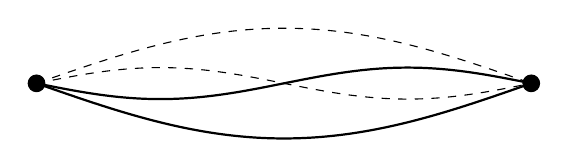
\begin{tikzpicture}[
tl/.style = {% tick labels
    fill=white, inner sep=1pt, font=\scriptsize,
            },                        ]

  \draw[dashed,draw=black,
      domain=-0:6.283,samples=300,variable=\x] 
      plot (\x,{0.7 * sin(deg{\x}/2)});
  \draw[thick,draw=black,
      domain=0:6.283,samples=300,variable=\x] 
  plot (\x,{0.7 * sin(deg{-1 * \x}/2)});
  
  \draw[dashed,draw=black,
      domain=-0:6.283,samples=300,variable=\x] 
      plot (\x,{0.2 * sin(deg{\x})});
  \draw[thick,draw=black,
      domain=0:6.283,samples=300,variable=\x] 
      plot (\x,{0.2 * sin(deg{-1 * \x})});

 \filldraw[black] (0, 0)  circle(3pt);
 \filldraw[black] (6.283, 0)  circle(3pt);

\end{tikzpicture}

The next overtone has two still points --- it divides the string into
three parts.  The outer parts are up, while the inner part is
down. Its frequency is three times the fundamental frequency.

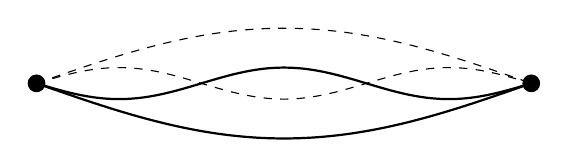
\begin{tikzpicture}[
tl/.style = {% tick labels
    fill=white, inner sep=1pt, font=\scriptsize,
            },                        ]

  \draw[dashed,draw=black,
      domain=-0:6.283,samples=300,variable=\x] 
      plot (\x,{0.7 * sin(deg{\x}/2)});
  \draw[thick,draw=black,
      domain=0:6.283,samples=300,variable=\x] 
  plot (\x,{0.7 * sin(deg{-1 * \x}/2)});
  
  \draw[dashed,draw=black,
      domain=-0:6.283,samples=300,variable=\x] 
      plot (\x,{0.2 * sin(1.5 * deg{\x})});
  \draw[thick,draw=black,
      domain=0:6.283,samples=300,variable=\x] 
      plot (\x,{0.2 * sin(1.5 * deg{-1 * \x})});

 \filldraw[black] (0, 0)  circle(3pt);
 \filldraw[black] (6.283, 0)  circle(3pt);

\end{tikzpicture}

And so on. 4 times the fundamental, 5 times the fundamental, etc.

In general, tones with many overtones tend to sound bright. Tones
with just the fundamental sound thin.

Humans can generally hear frequencies from 20Hz to 20,000Hz (or
20kHz).  Young people tend to be able to hear very high sounds better
than older people.

Dogs can generally hear sounds in the 65Hz to 45kHz range.

\section{Making waves in Python}

Let's make a sine wave and add some overtones to it.  Create a file named \filename{harmonics.py}.

\begin{Verbatim}
import matplotlib.pyplot as plt
import math

# Constants: frequency and amplitude
fundamental_freq = 440.0 # A = 440 Hz
fundamental_amp = 2.0

# Up an octave
first_freq = fundamental_freq * 2.0 # Hz
first_amp = fundamental_amp * 0.5

# Up a fifth more
second_freq = fundamental_freq * 3.0 # Hz
second_amp = fundamental_amp * 0.4

# How much time to show
max_time = 0.0092 # seconds

# Calculate the values 10,000 times per second
time_step = 0.00001 # seconds

# Initialize 
time = 0.0
times = []
totals = []
fundamentals = []
firsts = []
seconds = []

while time <= max_time:
    # Store the time
    times.append(time)
    
    # Compute value each harmonic
    fundamental = fundamental_amp * math.sin(2.0 * math.pi * fundamental_freq * time)
    first = first_amp * math.sin(2.0 * math.pi * first_freq * time)
    second = second_amp * math.sin(2.0 * math.pi * second_freq * time)

    # Sum them up
    total = fundamental + first + second

    # Store the values
    fundamentals.append(fundamental)
    firsts.append(first)
    seconds.append(second)
    totals.append(total)

    # Increment time
    time += time_step

# Plot the data
fig, ax = plt.subplots(2, 1)

# Show each component
ax[0].plot(times, fundamentals)
ax[0].plot(times, firsts)
ax[0].plot(times, seconds)
ax[0].legend()

# Show the totals
ax[1].plot(times, totals)
ax[1].set_xlabel("Time (s)")

plt.show()
\end{Verbatim}

When you run it, you should see a plot of all three sine waves and another plot of their sum:

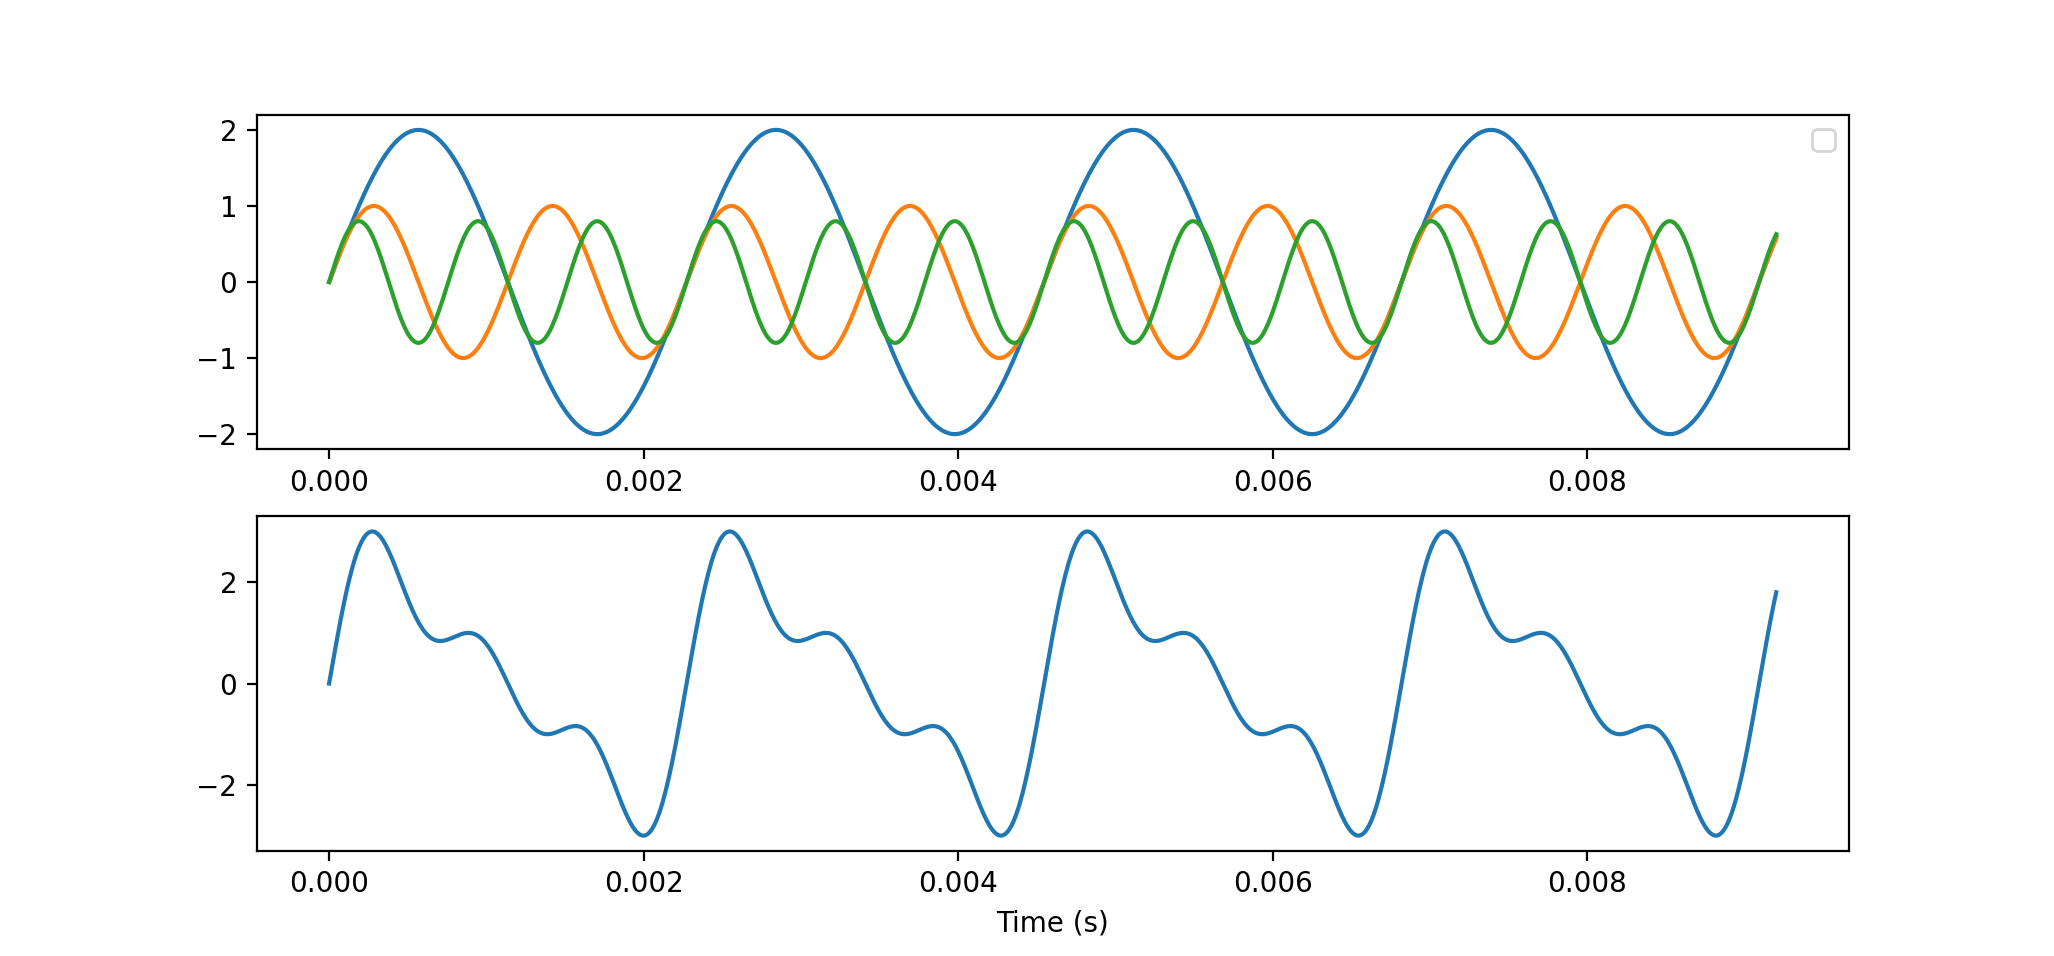
\includegraphics[width=0.9\linewidth]{harmonicspy.png}

\subsection{Making a sound file}

The graph is pretty to look at, but make let's a file that we can listen to.

The WAV audio file format is supported on pretty much any device, and
a library for writing WAV files comes with Python. Let's write some
sine waves and some noise into a WAV file.

Create a file called \filename{soundmaker.py}

\begin{Verbatim}
import wave
import math
import random

# Constants
frame_rate = 16000 # samples per second
duration_per = 0.3 # seconds per sound
frequencies = [220, 440, 880, 392] # Hz
amplitudes = [20, 125]
baseline = 127 # Values will be between 0 and 255, so 127 is the baseline
samples_per = int(frame_rate * duration_per) # number of samples per sound

# Open a file
wave_writer = wave.open('sound.wav', 'wb')

# Not stereo, just one channel
wave_writer.setnchannels(1)

# 1 byte audio means everything is in the range 0 to 255
wave_writer.setsampwidth(1)

# Set the frame rate
wave_writer.setframerate(frame_rate)

# Loop over the amplitudes and frequencies
for amplitude in amplitudes:
    for frequency in frequencies:
        time = 0.0
        # Write a sine wave
        for sample in range(samples_per):
            s = baseline + int(amplitude * math.sin(2.0 * math.pi * frequency * time))
            wave_writer.writeframes(bytes([s]))
            time += 1.0 / frame_rate
            
        # Write some noise after each sine wave
        for sample in range(samples_per):
            s = baseline + random.randint(0, 15)
            wave_writer.writeframes(bytes([s]))
            
# Close the file
wave_writer.close()
\end{Verbatim}

When you run it, it should create a sound file with several tones of
different frequencies and volumes. Each tone should be followed by
some noise.

\graphicspath{{../../Chapters/ac/en_US}}
\chapter{Alternating Current}

We have discussed the voltage and current created by a battery.  A
battery pushes the electrons in one direction at a constant voltage;
this is known as \newterm{Direct Current} or DC. A battery typically
provides between 1.5 and 9 volts.

The electrical power that comes into your home on wires is
different. If you plotted the voltage over time, it would look like
this:

\begin{tikzpicture}[
tl/.style = {% tick labels fill=white, inner sep=1pt,
  font=\scriptsize, }, ]
% grid
\draw[sdkblue, very thin, xstep=0.5235, ystep=0.425] (0,-1.85) grid
(6.6,1.85);

% y tick label
\foreach \y in {-170, -85, 85, 170}{\node[tl,left=1mm] at (0,{\y/100})
  {$\y$};}

% x tick label
\foreach \x in {0.004,0.008, 0.012, 0.016}{\node[tl,below=1mm] at
  ({392.67*\x},0) {$\x$};}

% axes
\draw[->,thick] (0,0) -- (6.5,0) node[right] {$seconds$};
\draw[->,thick] (0,-1.8) -- (0, 1.8) node[above] {$volts$};
% curve
\draw[<->,thick,draw=black,domain=0:6.5,samples=300,variable=\x] plot
(\x,{sin(deg(\x)) * 1.7});
\end{tikzpicture}

The $x$ axis here represents ground. When you insert a two-prong plug
into an outlet, one is ``hot'' and the other is ``ground''. Ground
represents 0 volts and should be the same voltage as the dirt under
the building.

The voltage is a sine wave at 60Hz. Your voltage fluctuates between
-170v and 170v. Think for a second what that means: The power company
pushes electrons at 170v and then pulls electrons at 170v.  It
alternates back and forth this way 60 times per second.

\section{Power of AC}

Let's say you turn on your toaster which has a resistance of 14.4
ohms. How much energy (in watts) does it change from electrical energy
to heat?  We know that $I = V/R$ and we know that watts of power is
$IV$. So given a voltage of $V$, the toaster is consuming $V^2/R$
watts.

However, $V$ is fluctuating. Let's plot the power the toaster is consuming:

\begin{tikzpicture}[
tl/.style = {% tick labels
    fill=white, inner sep=1pt, font=\scriptsize,
            },                        ]
% grid
\draw[sdkblue, very thin, xstep=0.5235, ystep=0.5] (0,0) grid (6.6,2.1);

% y tick label
\foreach \y in {500, 1000, 1500, 2000}{\node[tl,left=1mm] at (0,{\y/1000}) {$\y$};}

% x tick label
\foreach \x in {0.004,0.008, 0.012, 0.016}{\node[tl,below=1mm] at ({392.67*\x},0) {$\x$};}

% axes
\draw[->,thick] (0,0) -- (6.5,0) node[right] {$seconds$};
\draw[->,thick] (0,0) -- (0, 2.1) node[above] {$watts$};
% curve
\draw[<->,thick,draw=black,domain=0:6.5,samples=300,variable=\x]
      plot (\x,{sin(deg(\x))^2 * 2.007});
\end{tikzpicture}

Another sine wave! Here is a lesser-known trig identity: $\left( \sin(x) \right)^2 = \frac{1}{2} - \frac{1}{2}\cos(2x)$

So this is actually a cosine wave flipped upside down, scaled down by
half the peak power and translated up so that it is never
negative. Note that it is also twice the frequency of the voltage sine
wave.

If we say the peak voltage is $V_p$ and the resistance of the toaster
is $R$, the power is given by

$$\frac{V_p^2}{2R} - \frac{V_p^2}{2R} \cos \left(\frac{2\pi t}{120} \right)$$

As a toaster user and as someone who pays a power bill, you are mostly
interested in the average power.  To get the average power, you take
the area under the power graph and divide it by the amount of time.

We can think of the area under the curve as two easy-to-integrate quantites summed:
\begin{itemize}
\item A constant function of $y = frac{V_p^2}{2R}$
\item A wave $y = - \frac{V_p^2}{2R} \cos \left(\frac{2\pi t}{120} \right)$
\end{itemize}

\begin{tikzpicture}[
tl/.style = {% tick labels
    fill=white, inner sep=1pt, font=\scriptsize,
            },                        ]
% grid
\draw[sdkblue, very thin, xstep=0.5235, ystep=0.5] (0,-1.1) grid (6.6,1.1);

% y tick label
\foreach \y in {-1000, -500, 500, 1000}{\node[tl,left=1mm] at (0,{\y/1000}) {$\y$};}

% x tick label
\foreach \x in {0.004,0.008, 0.012, 0.016}{\node[tl,below=1mm] at ({392.67*\x},0) {$\x$};}

% axes
\draw[->,thick] (0,0) -- (6.5,0) node[right] {$seconds$};
\draw[<->,thick] (0,-1.1) -- (0, 1.1) node[above] {$watts$};
% curve
\draw[<->,thick,draw=black] (0,1.003) -- (6.5, 1.003) node[right] {Constant: $\frac{V_p^2}{2R}$};
\draw[<->,thick,draw=black,domain=0:6.5,samples=300,variable=\x]
      plot (\x,{-1 * cos(deg(\x) * 2) * 1.003}) node[right]{Wave:$- \frac{V_p^2}{2R} \cos \left(\frac{2\pi t}{120} \right)$};
\end{tikzpicture}
    
When we integrate that constant function we get $\frac{t V_p^2}{2R}$

When we integrate that wave for a complete cycle we get...zero! The
positive side of the wave is canceled out by the negative side.

So, the average power is $\frac{V_p^2}{2R}$ watts.

Someone at some point said ``I'm used to power being $V^2/R$. Can
we define a voltage measure for AC power such that this is always true?''

So we started using $V_{rms}$ which is just
$\frac{V_p}{\sqrt{2}}$. If you look on the back of anything that plugs
into a standard US power outlet, it will say something like ``For
120v''.  What they mean is ``For 120v RMS, so we expect the voltage to
fluctuate back and forth from 170v to -170v.''

Notice that this is the same Root-Mean-Squared that we defined
earlier, but now we know that if $y = \sin(x)$, the RMS of $y$ is
$1/\sqrt{2} \approx 0.707$.

For current, we do the same thing: If the current is AC, the power
consumed by a resistor is $I_{RMS}^2 R$, where $I_{RMS}$ is the peak
current divided by $sqrt{2}$.

\section{Power Line Losses}

A wire has some resistance. Thinner wires tend to have more resistance
than thicker ones. Aluminum wires tend to have more resistance than
copper wires.

Let's say that the power that comes to your house has to travel 20 km
from the generator in a cable that has about $1 \Omega$ of resistance
per km.  Let's say that your home is consuming 12 kilowatts of power.

If that power is 120v RMS from the generator to your home, what
percentage of the power is lost heating the power line? 10 amps RMS
flow through your home. When that current goes through the wire, $I^2
R = (100)(20) = 2000 watts$ is lost to heat.

So the power company would need to supply 14 kilowatts of power,
knowing that 2 kilowatts would be lost on the wires.

What if the power company moved the power at 120,000 volts RMS? Now
only 0.01 amps RMS flow through your home. When that current goes
through the wire $I^2R = (0.0001)(20) = .002$ watts of power are lost
on the power lines.

It is much, much more efficent. The only problem is that 120,000 volts
would be incredibly dangerous.  So the power company moves power long
distances at very high voltages, like 765 kV.  Before the power is
brought into your home, it is converted into a lower voltage using a
\newterm{transformer}.

\section{Transformers}

A transformer is a device that converts electrical power from one
voltage to another. A good tranformer is more than 95\% efficient. The
details of magnetic fields, flux, and inductance are beyond this scope
of this chapter, so I am going to give a relatively simple explanation
and admit that it is incomplete.

A transformer is a ring with two sets of coils wrapped around it.

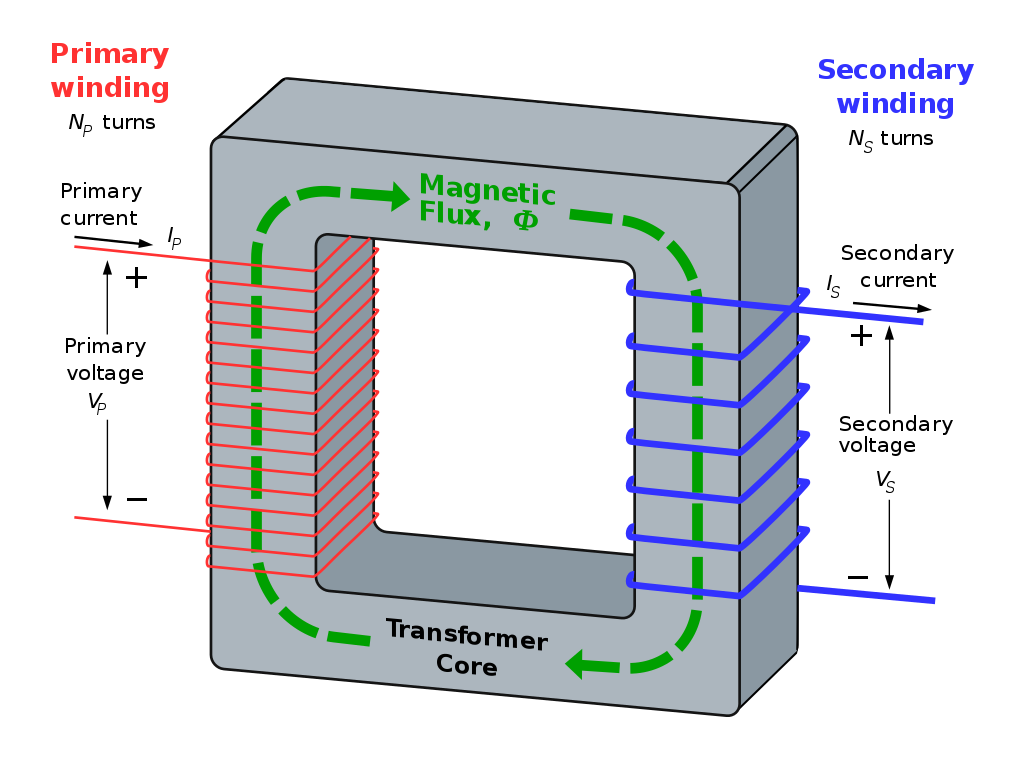
\includegraphics[width=0.5\textwidth]{transformer.png}

(Diagram from Wikipedia)

When AC current is run through the primary winding, it create magnetic
flux in the ring.  The magnetic flux induces current in the secondary
winding.

If $V_P$ is the voltage across the primary winding and $V_S$ is the
voltage across the secondary winding, they are related by the
following equation:

$$\frac{V_P}{V_S} = \frac{N_P}{N_S}$$

where $N_P$ and $N_S$ are the number of turns in the primary and
secondary windings.

There are usually at least two transformers between you and the very
high voltage lines.  There are tranformers at the substation that make
the voltage low enough to travel on regular utility poles. On the
utility poles, you will see cans that contain smaller
transformers. Those step the voltage down to make the power safe to
enter your home.

\section{Phase and 3-phase power}

If two waves that are ``in sync'' we say they have the same \newterm{phase}.

\begin{tikzpicture}[
tl/.style = {% tick labels fill=white, inner sep=1pt,
  font=\scriptsize, }, ]
% grid
\draw[sdkblue, very thin, xstep=0.5235, ystep=0.425] (0,-1.85) grid
(13,1.85);

% axes
\draw[->,thick] (0,0) -- (13,0);
% curve
\draw[thick,draw=black,domain=0:13,samples=500,variable=\x] plot
(\x,{sin(deg(\x)) * 1.7});
\draw[thick,dashed, draw=black,domain=0:13,samples=500,variable=\x] plot
(\x,{sin(deg(\x)) * 0.9});
\end{tikzpicture}

If they are the same frequency, but are not in-sync, we can talk about
the difference in their phase.

\begin{tikzpicture}[
tl/.style = {% tick labels fill=white, inner sep=1pt,
  font=\scriptsize, }, ]
% grid
\draw[sdkblue, very thin, xstep=0.5235, ystep=0.425] (0,-1.85) grid
(13,1.85);

% axes
\draw[->,thick] (0,0) -- (13,0);
% curve
\draw[thick,draw=black,domain=0:13,samples=500,variable=\x] plot
(\x,{sin(deg(\x)) * 1.7});
\draw[thick,dashed, draw=black,domain=0:13,samples=500,variable=\x] plot
(\x,{sin(deg(\x) - 90) * 0.9});
\end{tikzpicture}

Here we see that the smaller wave is lagging by $\pi/2$ or $90^\circ$.

In most power grids, there are usually 3 wires carrying the power.
The voltage on each is $2\pi/3$ out of phase with the other two:

\begin{tikzpicture}[
tl/.style = {% tick labels fill=white, inner sep=1pt,
  font=\scriptsize, }, ]
% grid
\draw[sdkblue, very thin, xstep=0.5235, ystep=0.425] (0,-1.85) grid
(13,1.85);

% axes
\draw[->,thick] (0,0) -- (13,0);
% curve
\draw[thick,draw=black,domain=0:13,samples=500,variable=\x] plot
(\x,{sin(deg(\x)) * 1.7});
\draw[thick,dashed, draw=black,domain=0:13,samples=500,variable=\x] plot
(\x,{sin(deg(\x) - 120) * 1.7});
\draw[thick,draw=sdkblue,domain=0:13,samples=500,variable=\x] plot
(\x,{sin(deg(\x) + 120) * 1.7});
\end{tikzpicture}

This is nice in two ways:
\begin{itemize}
\item While the power in each wire is fluctuating, the total power is not fluctuating at all.
\item While the power plant is pushing and pulling electrons on each
  wire, the total number number of electrons leaving the load is zero.
\end{itemize}
(Both these assume that there each wire is attached to a load with the same constant resistance.)

In big industrial factories, you will see all three wires enter the
building. Large amounts of smooth power delivery means a lot to an
industrial user.

In residential settings, each home gets its power from one of the three
wires. However two wires typically carry power into the home. Each
one carries 120V RMS, but they are out of phase by 180 degree. Lights
and small appliances are connected to one of the wires and ground, so
they get 120V RMS.  Large appliances, like air conditioners and
washing machines, are connected across the two wires so they get 240V
RMS.

\begin{tikzpicture}[
tl/.style = {% tick labels fill=white, inner sep=1pt,
  font=\scriptsize, }, ]
% grid
\draw[sdkblue, very thin, xstep=0.5235, ystep=0.425] (0,-1.85) grid
(13,1.85);

% axes
\draw[->,thick] (0,0) -- (13,0);
% curve
\draw[thick,draw=black,domain=0:13,samples=500,variable=\x] plot
(\x,{sin(deg(\x)) * 1.7});
\draw[thick,dashed, draw=black,domain=0:13,samples=500,variable=\x] plot
(\x,{sin(deg(\x) + 180) * 1.7});
\draw[<->, thick, draw=black] (7.85398, 0) -- (7.85398, 1.7) node [midway, right] {120V};
\draw[<->, thick, draw=black] (4.712, -1.7) -- (4.712, 1.7);
\draw (4.712, 0.8) node[right] {240V};
\end{tikzpicture}


How do you get two circuits, 180 degrees out of phase, from one
circuit?  Using a center-tap transformer.

FIXME: Diagram here





\graphicspath{{../../Chapters/drag/en_US}}
\chapter{Drag}

The very first computers were created to do calculations of how
artillery would fly when shot at different angles. The calculations
were similar to the ones you just did for the flying
hammer with two important differences:
\begin{itemize}
\item They were interested in two dimensions: the height and the distance across the ground.
\item However, artillery flies a lot faster than a hammer, so they had to worry about drag from the air.
\end{itemize}
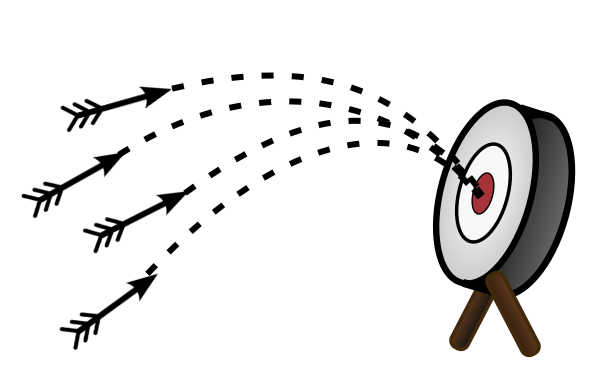
\includegraphics[width=0.8\textwidth]{arrows.png}
\section{Wind resistance}

The first thing they did was put one of the shells in a wind tunnel.
They measured how much force was created when they pushed 1 m/s of
wind over the shell. Let's say it was 0.1 newtons.

One of the interesting things about the drag from the air (often
called \newterm{wind resistance}) is that it increases with the
\emph{square} of the speed. Thus, if the wind pushing on the shell is
3 m/s, instead of 1 m/s, the resistance is $3^2 \times 0.1 = 0.9$
newtons.

(Why? Intuitively, three times as many air molecules are hitting the
shell and each molecule is hitting it three times harder.)

So, if a shell is moving with the velocity vector $v$, the force
vector of the drag points in the exact opposite direction. If $\mu$ is
the force of wind resistance of the shell at 1 m/s, then the magnitude
of the drag vector is $\mu |v|^2$.

\section{Initial velocity and acceleration due to gravity}

Let's say a shell is shot out of a tube at $s$ m/s, and let's say the tube
is tilted $\theta$ radians above level.  Then, the initial velocity
will be given by the vector $[s \cos(\theta), s \sin(\theta)]$

(The velocity of the shell is actually a 3-dimensional vector, but we
are only going to worry about height and horizontal distance; we are
assuming that the operator pointed it in the right direction.)

To figure out the path of the shell, we need to compute its acceleration. We remember that

$$F = m a$$

(Note that $F$ and $a$ are vectors.)  Dividing both sides by $m$ we get:

$$a = \frac{F}{m}$$

So let's figure out the net force on the shell so that we can calculate the acceleration vector.

If the shell has a mass of $b$, the force due to gravity will be in the
downward direction with a magnitude of $9.8 b$ newtons.

To get the net force, we will need to add the force due to gravity
with the force due to wind resistance.

\section{Simulating artillery in Python}

Create a file called \filename{artillery.py}.

\begin{Verbatim}
    import numpy as np
    import matplotlib.pyplot as plt
    
    # Constants
    mass = 45 # kg
    start_speed = 300.0 # m/s
    theta = np.pi/5 # radians (36 degrees above level)
    time_step = 0.01 # s
    wind_resistance = 0.05 # newtons in 1 m/s wind
    force_of_gravity = np.array([0.0, -9.8 * mass]) # newtons
    
    # Initial state
    position = np.array([0.0, 0.0]) # [distance, height] in meters
    velocity = np.array([start_speed * np.cos(theta), start_speed * np.sin(theta)])
    time = 0.0 # seconds
    
    # Lists to gather data
    distances = []
    heights = []
    times = []
    
    # While shell is aloft
    while position[1] >= 0:
        # Record data
        distances.append(position[0])
        heights.append(position[1])
        times.append(time)
    
        # Calculate the next state
        time += time_step
        position += time_step * velocity
    
        # Calculate the net force vector
        force = force_of_gravity - wind_resistance * velocity**2
    
        # Calculate the current acceleration vector
        acceleration = force / mass
    
        # Update the velocity vector   
        velocity += time_step * acceleration
    
    print(f"Hit the ground {position[0]:.2f} meters away at {time:.2f} seconds.")
    
    # Plot the data
    fig, ax = plt.subplots()
    ax.plot(distances, heights)
    ax.set_title("Distance vs. Height")
    ax.set_xlabel("Distance (m)")
    ax.set_ylabel("Height (m)")
    plt.show()        
\end{Verbatim}

When you run it, you should get a message like:
\begin{Verbatim}
Hit the ground 1696.70 meters away at 20.73 seconds.
\end{Verbatim}

You should also see a plot of the shell's path:

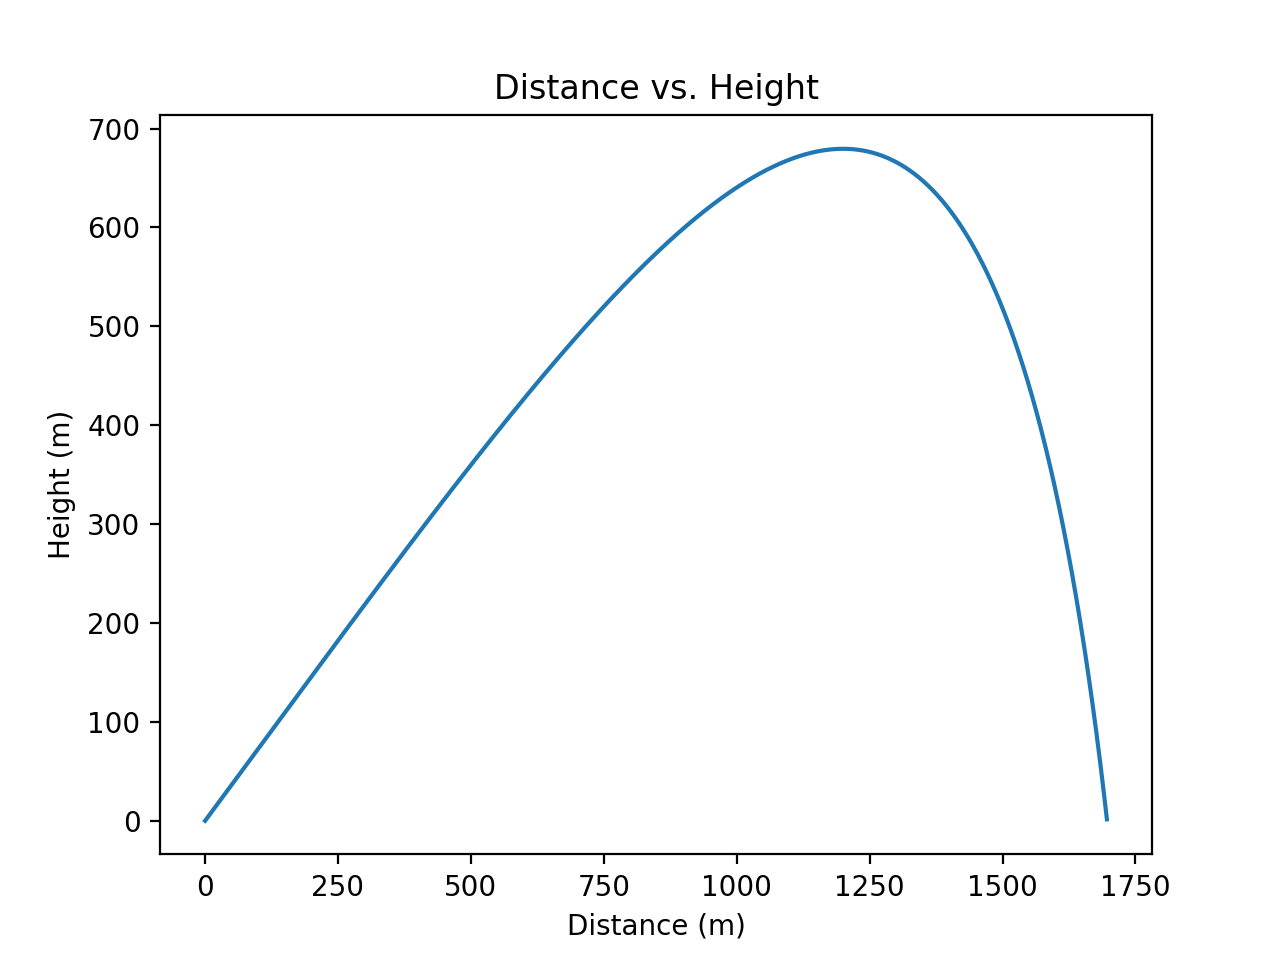
\includegraphics[width=0.8\textwidth]{artillery.png}

\section{Terminal velocity}

If you shot the shell very, very high in the sky, it would keep accelerating 
toward the ground until the force of gravity and the force of the wind resistance were equal.
The speed at which this happens is called the \newterm{terminal velocity}.  The terminal velocity of a
falling human is about 53 m/s.

\begin{Exercise}[title={Terminal velocity}, label=terminal_velocity]
    What is the terminal velocity of shell described in our example?
\end{Exercise}
\begin{Answer}[ref=terminal_velocity]
The force of gravity is $9.8 \times 45 = 441$ newtons.

At any speed $s$, the force of wind resistance is $0.05 \times s^2 = 0.05 s^2$ newtons.

At terminal velocity, $0.05 s^2 = 441$. 

Solving for $s$, we get $s = \sqrt{\frac{441}{0.05}}$

Thus, terminal velocity should be about 94 m/s.

\end{Answer}

\graphicspath{{../../Chapters/vector_functions/en_US}}
\chapter{Vector-valued Functions}

In the last chapter, you calculated the flight of the shell.  For any
time $t$, you could find a vector $[distance, height]$. This can be
thought of as a function $f$ that takes a number and returns a
2-dimensional vector.  We call this a \newterm{vector-valued} function
from $\mathbb{R} \rightarrow \mathbb{R}^2$.
% Define the R symbol

We often make a vector-valued function by defining several real-valued
functions.  For example, if you threw a hammer with an initial upward
speed of 12 m/2 and a horizontal speed of 4 m/s along the $x$ axis from
the point $(1, 6, 2)$, its position at time $t$ (during its flight) would be given by:
% Format 12/ m2
$$f(t) = [4t + 1, 6, -4.8t^2 + 12t + 2]$$

That is, $x$ is increasing with $t$, $y$ is constant, and $z$ is a parabola.

\tdplotsetmaincoords{80}{20} 
\begin{tikzpicture} [scale=0.5, tdplot_main_coords, axis/.style={->,sdkblue}, 
vector/.style={-stealth,black,very thick}, 
vector guide/.style={dashed,sdkblue}]

%standard tikz coordinate definition using x, y, z coords
\coordinate (O) at (0,0,0);

%draw axes
\draw[axis] (0,0,0) -- (12,0,0) node[anchor=north east]{$x$};
\draw[axis] (0,0,0) -- (0,7,0) node[above]{$y$};
\draw[axis] (0,0,0) -- (0,0,10) node[anchor=south]{$z$};

\draw[thick,draw=black,
      domain=0:2.60563,samples=300,variable=\t] 
      plot ({4*\t + 1},6, {-4.9*\t^2 + 12*\t + 2});
\draw[dashed,draw=sdkblue] (1, 6, 0) -- (11.42252, 6, 0);
\draw[dashed,draw=sdkblue] (11.42252, 0, 0) -- (11.42252, 6, 0);
\draw[dashed,draw=sdkblue] (1, 6, 0) -- (1, 6, 2);
\draw[dashed,draw=sdkblue] (1, 6, 0) -- (1, 6, 2);
\draw[dashed,draw=sdkblue] (1, 6, 0) -- (1, 0, 0);

\filldraw[black] (1,6,2) circle(4pt) node [left]{$f(0) = [1,6,2]$};
\filldraw[black] (5,6,9.1) circle(4pt) node [above]{$f(1) = [5, 6, 9.1]$};
\draw[dashed,draw=sdkblue] (5, 6, 0) -- (5, 6, 9.1);
\filldraw[black] (9,6,6.4) circle(4pt) node [right]{$f(2) = [9, 6, 6.4]$};
\draw[dashed,draw=sdkblue] (9, 6, 0) -- (9, 6, 6.4);
\filldraw[black] (11.42252,6,0) circle(4pt) node [right] {$f(2.6) = [11.4, 6, 0]$};
\end{tikzpicture}

\section{Finding the velocity vector}


Now that we have its position vector, we can differentiate each
component separately to get its velocity as a vector-valued function:

$$f'(t) = [4, 0, -9.8t + 12]$$

That is, the velocity is constant along the $x$-axis, zero along the
$y$-axis, and decreasing with time along the $z$ axis.

\tdplotsetmaincoords{80}{20} 
\begin{tikzpicture} [scale=0.5, tdplot_main_coords, axis/.style={->,sdkblue}, 
vector/.style={-stealth,black,very thick}, 
vector guide/.style={dashed,sdkblue}]

%standard tikz coordinate definition using x, y, z coords
\coordinate (O) at (0,0,0);

%draw axes
\draw[axis] (0,0,0) -- (14,0,0) node[anchor=north east]{$x$};
\draw[axis] (0,0,0) -- (0,7,0) node[above]{$y$};
\draw[axis] (0,0,0) -- (0,0,10) node[anchor=south]{$z$};

\draw[thick,dashed,draw=black,
      domain=0:2.60563,samples=300,variable=\t] 
      plot ({4*\t + 1},6, {-4.9*\t^2 + 12*\t + 2});

\filldraw[black] (1,6,2) circle(4pt);
\draw[->, thick, draw=black] (1,6,2) -- (5, 6, 14) node [right] {$f'(0) = [4,0,12]$};
\draw[dashed, draw=sdkblue] (1,6,2) -- (5,6,2) -- (5,6,14);
\filldraw[black] (5,6,9.1) circle(4pt);
\draw[->, thick, draw=black] (5,6,9.1) -- (9, 6, 11.3) node [right] {$f'(1) = [4,0,2.2]$};
\draw[dashed, draw=sdkblue] (6,6,9.1) -- (9,6,9.1) -- (9,6,11.3);
\filldraw[black] (9,6,6.4) circle(4pt);
\draw[->, thick, draw=black] (9,6,6.4) -- (13, 6, -1.2) node [right] {$f'(2) = [4,0,-7.6]$};
\filldraw[black] (11.42252,6,0) circle(4pt);
\draw[dashed, draw=sdkblue] (9,6,6.4) -- (13,6,6.4) -- (13,6,-1.2);
\end{tikzpicture}


\section{Finding the acceleration vector}


Now that we have its velocity, we can get its acceleration as a vector-valued function:

$$f''(t) = [0, 0, -9.8]$$

There is no acceleration along the $x$ or $y$ axes. It is accelerating
down at a constant $9.8 m/s^2$.

\tdplotsetmaincoords{80}{20} 
\begin{tikzpicture} [scale=0.5, tdplot_main_coords, axis/.style={->,sdkblue}, 
vector/.style={-stealth,black,very thick}, 
vector guide/.style={dashed,sdkblue}]

%standard tikz coordinate definition using x, y, z coords
\coordinate (O) at (0,0,0);

%draw axes
\draw[axis] (0,0,0) -- (14,0,0) node[anchor=north east]{$x$};
\draw[axis] (0,0,0) -- (0,7,0) node[above]{$y$};
\draw[axis] (0,0,0) -- (0,0,10) node[anchor=south]{$z$};

\draw[thick,dashed,draw=black,
      domain=0:2.60563,samples=300,variable=\t] 
      plot ({4*\t + 1},6, {-4.9*\t^2 + 12*\t + 2});

\filldraw[black] (1,6,2) circle(4pt);
\draw[->, thick, draw=black] (1,6,2) -- (1, 6, -7.8) node [right] {$f''(0) = [0,0,-9.8]$};
\filldraw[black] (5,6,9.1) circle(4pt);
\draw[->, thick, draw=black] (5,6,9.1) -- (5, 6, -0.7) node [below] {$f''(1) = [0,0,-9.8]$};
\filldraw[black] (9,6,6.4) circle(4pt);
\draw[->, thick, draw=black] (9,6,6.4) -- (9, 6, -3.4) node [right] {$f''(2) = [0,0,-9.8]$};
\filldraw[black] (11.42252,6,0) circle(4pt);
\end{tikzpicture}


\graphicspath{{../../Chapters/circular/en_US}}
\chapter{Circular Motion}

Let's say you tie a 0.16 kg billard ball to a long string and begin to swing
it around in a circle above your head. The string is 3
meters long, and the ball returns to where it started every 4
seconds. If you start your stopwatch as the ball crosses the
$x$-axis, the position of the ball at any time $t$ given by:

$$p(t) = [3 \cos{\left( \frac{2 \pi} {4}t\right)}, 3 \sin{ \left( \frac{2 \pi}{4}t\right) }, 2]$$

(This assumes that the ball would be going counter-clockwise if viewed
from above. The spot you are standing on is considered the origin $[0, 0, 0]$.)

Notice that the height is a constant --- 2 meters in this
case. That isn't very interesting, so we will talk just about the
first two components.  Here is what it would look like from above:

% 3sin = 1.267854785222098
% 3cos = 2.71892336110995
\begin{tikzpicture}[declare function={angle=25;},bullet/.style={inner
    sep=1pt,fill,draw,circle,solid}, scale=1.7]
    % Axis
    \draw[thick,-stealth,black] (-3.2,0)--(3.2,0) node[right] {$x$}; % x axis
    \draw[thick,-stealth,black] (0,-3.2)--(0,3.2) node[left] {$y$}; % y axis
    % Rest
    \draw [dashed, sdkblue] (0,0) circle (3);
    \draw[thick] (0,0) -- (angle:3.0) node [midway, above] {3};
    \draw[sdkblue] (1.05, 0.2) node[right] {$\theta = \frac{2\pi t}{4}\text{ radians}$};
    \draw[-stealth,sdkblue] (1,0) arc (0:angle:1);
    \draw[dashed, black] (2.71892336110995, 1.267854785222098) -- (2.71892336110995, 0)
    node[below] {$3 \cos(\theta)$}; % vertical
    \draw[dashed, black] (2.71892336110995, 1.267854785222098) -- (0, 1.267854785222098)
    node[left] {$3 \sin(\theta)$}; % horizontal
    \filldraw[black] (angle:3.0) circle(4pt);
    \draw[->, thick] (2.71892336110995, 1.267854785222098) --
    (2.71892336110995 - 3 * 0.1267, 1.267854785222098 + 3 * 0.2718);
\end{tikzpicture}

In this case, the radius, $r$, is 3 meters.  The period, $T$, is 4
seconds.  In general, we say that circular motion is given by:

$$p(t) = \left[ r \cos{\frac{2 \pi t}{T}}, r \cos{\frac{2 \pi t}{T}}\right]$$

A common question is ``How fast is it turning right now?''  If you
divide the $2\pi$ radians of a circle by the 4 seconds it takes, you
get the answer ``About 1.57 radians per second.''  This is known as
\newterm{angular velocity} and we typically represent it with the
lowercase Omega: $\omega$. (Yes, it looks a lot like a ``w''.)  To be
precise, in our example, the angular velocity is $\omega = \frac{\pi}{2}$.

Notice that this is different from the question ``How fast is it
going?''  This ball is traveling the circumference of $6\pi \approx
18.85$ meters every 4 seconds.  This means the speed of the ball is about
4.71 meters per second.

\section{Velocity}

The velocity of the ball is a vector, and we can find that vector by
differentiating each component of the position vector.

For any constants $a$ and $b$:

\begin{tabular}{c | c }
  Expression & Derivative \\
  \hline
  $a \sin{b t}$ & $ab \cos{b t}$ \\
  $a \cos{b t}$ & $-ab \sin{b t}$  \\
\end{tabular}

Thus, in our example, the velocity of the ball at any time $t$ is given by:

$$v(t) = \left[ -\frac{3 (2\pi)}{4} \sin{\frac{2\pi t}{4}}, \frac{3(2\pi)}{4} \cos{\frac{2\pi t}{4}}, 0 \right]$$

Notice that the velocity vector is perpendicular to the position vector.  It has a constant magnitude.

In general, an object traveling in a circle at a constant speed has the velocity vector:

$$v(t) = \left[ -r\omega \sin{\omega t}, r\omega \cos{\omega t}\right]$$

where $t = 0$ is the time that it crosses the $x$ axis.  If \omega is
negative, that means the motion would be clockwise when viewed from
above.

The magnitude of the velocity vector is $r\omega$. 

\begin{tikzpicture}[declare function={angle=25;},bullet/.style={inner
    sep=1pt,fill,draw,circle,solid}, scale=1.7]
    % Axis
    \draw[thick,-stealth,black] (-3.2,0)--(3.2,0) node[right] {$x$}; % x axis
    \draw[thick,-stealth,black] (0,-3.2)--(0,3.2) node[left] {$y$}; % y axis
    % Rest
    \draw [dashed, sdkblue] (0,0) circle (3);
    \filldraw[black] (angle:3.0) circle(4pt);
    \draw[->, thick] (2.71892336110995, 1.267854785222098) --
    (2.71892336110995 - 0.6 * 1.267, 1.267854785222098 + 0.6 * 2.718) node[right]{$v(t)=\left[ -r\omega \sin{\omega t}, r\omega \cos{\omega t}\right]$};
\end{tikzpicture}

\section{Acceleration}

We can get the acceleration by differentiating the components of the velocity vector.

$$a(t) = \left[-r \omega^2 \cos{\omega t}, -r \omega^2 \sin{\omega t} \right]$$

Notice that the acceleration vector points toward the center of the
circle it is traveling on.  That is, when an object is traveling on a
circle at a constant speed, its only acceleration is toward the center
of the circle.

\begin{tikzpicture}[declare function={angle=25;},bullet/.style={inner
    sep=1pt,fill,draw,circle,solid}, scale=1.7]
    % Axis
    \draw[thick,-stealth,black] (-3.2,0)--(3.2,0) node[right] {$x$}; % x axis
    \draw[thick,-stealth,black] (0,-3.2)--(0,3.2) node[left] {$y$}; % y axis
    % Rest
    \draw [dashed, sdkblue] (0,0) circle (3);
    \filldraw[black] (angle:3.0) circle(4pt);
    \draw[->, thick] (2.71892336110995, 1.267854785222098) --
    (2.71892336110995 * 0.2 , 1.267854785222098 * 0.2) node[midway, right]{$a(t) = \left[-r \omega^2 \cos{\omega t}, -r \omega^2 \sin{\omega t} \right]$};
\end{tikzpicture}

The magnitude of the acceleration vector is $r \omega^2$.

\section{Centripetal force}

How hard is the ball pulling against your hand?  That is, if you let
go, the ball would fly in a straight line.  The force you are exerting
on the string is what causes it to accelerate toward the center of the
circle. We call this the \newterm{centripetal force}.

Recall that $F = m a$.  The magnitude of the acceleration is $r
\omega^2 = 3 \left(\frac{2 pi}{4}\right)^2 \approx 7.4$ m/s.  The mass
of the ball is 0.16 kg.  So, the force pulling against your hand is
about 1.18 newtons.

The general rule is that when something is traveling in a circle at a
constant speed, the centripetal force needed to keep it traveling in a
circle is:

$$F = m r \omega^2$$

If you know the radius $r$ and the speed $v$ of the object, here is the rule:

$$F = \frac{m v^2}{r}$$

\begin{Exercise}[title={Circular Motion}, label=circular]
Just as your car rolls onto a circular track with a radius of 200 m,
you realize your 0.4 kg cup of coffee is on the slippery dashboard of your
car.  While driving 120 km/hour, you hold the cup to keep it from sliding.

What is the maximum amount of force you would need to use? (The friction of
the dashboard helps you, but the max is when the friction is zero.)

\end{Exercise}
\begin{Answer}[ref=circular]
  $$\frac{120 \text{ km}}{1 hour} = \frac{1000 \text{ m}}{1 \text{ km}}\frac{120 \text{ km}}{1 hour} \frac{1 \text{ hour}}{3600 \text{ seconds}}= 33.3 \text{ m/s}$$

  $$F = \frac{m v^2}{r} = \frac {0.4 (33.3)^2}{200} = 2.2 \text{ newtons}$$
\end{Answer}

\graphicspath{{../../Chapters/orbits/en_US}}
\chapter{Orbits}

A satellite stays in orbit around the planet because the pull of the
planet's gravity causes it to accelerate toward the center of the
planet. 

\begin{figure}[htbp]
    \centering
    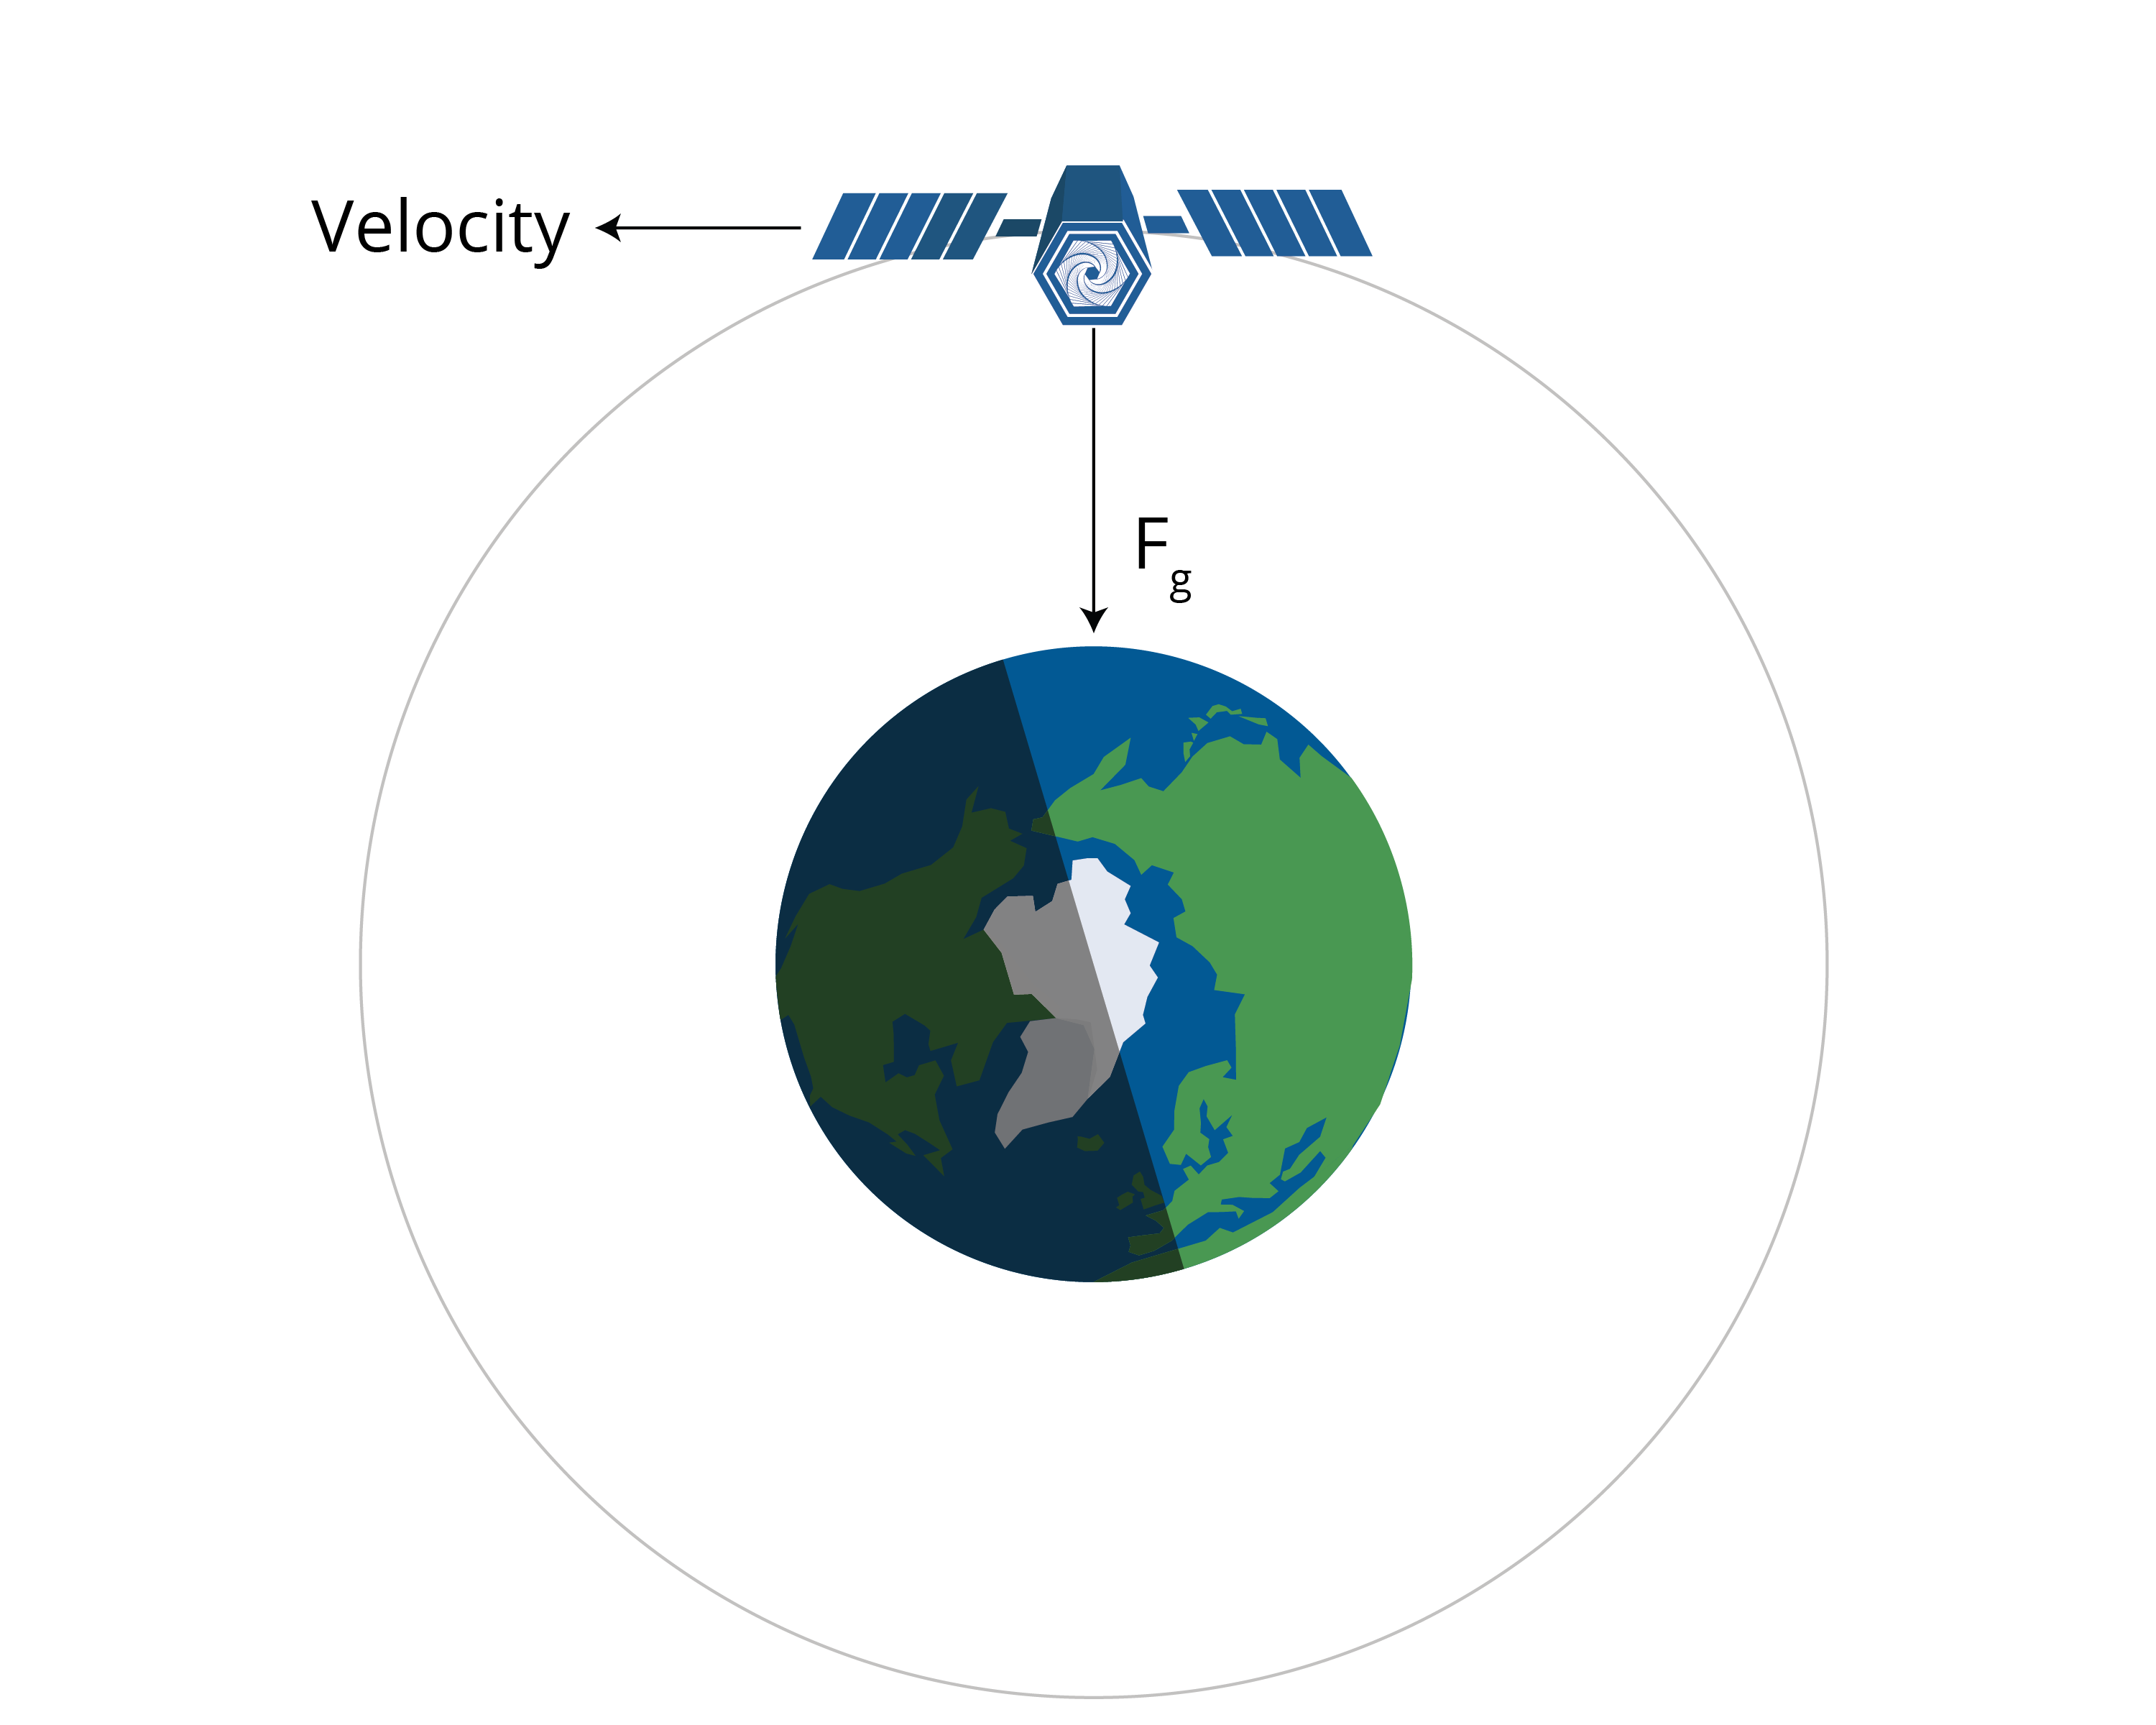
\includegraphics[width=.75\textwidth]{satellite.png}
    \caption{A satellite's centripetal force is gravity.}
    \label{fig:satellite}
\end{figure}


The satellite must be moving at a very particular speed to keep a
constant distance from the planet --- to travel in a circular orbit.
If it is moving too slowly, it will get closer to the planet.  If it
is going too fast, it will get farther from the planet.
\begin{figure}[htbp]
    \centering
    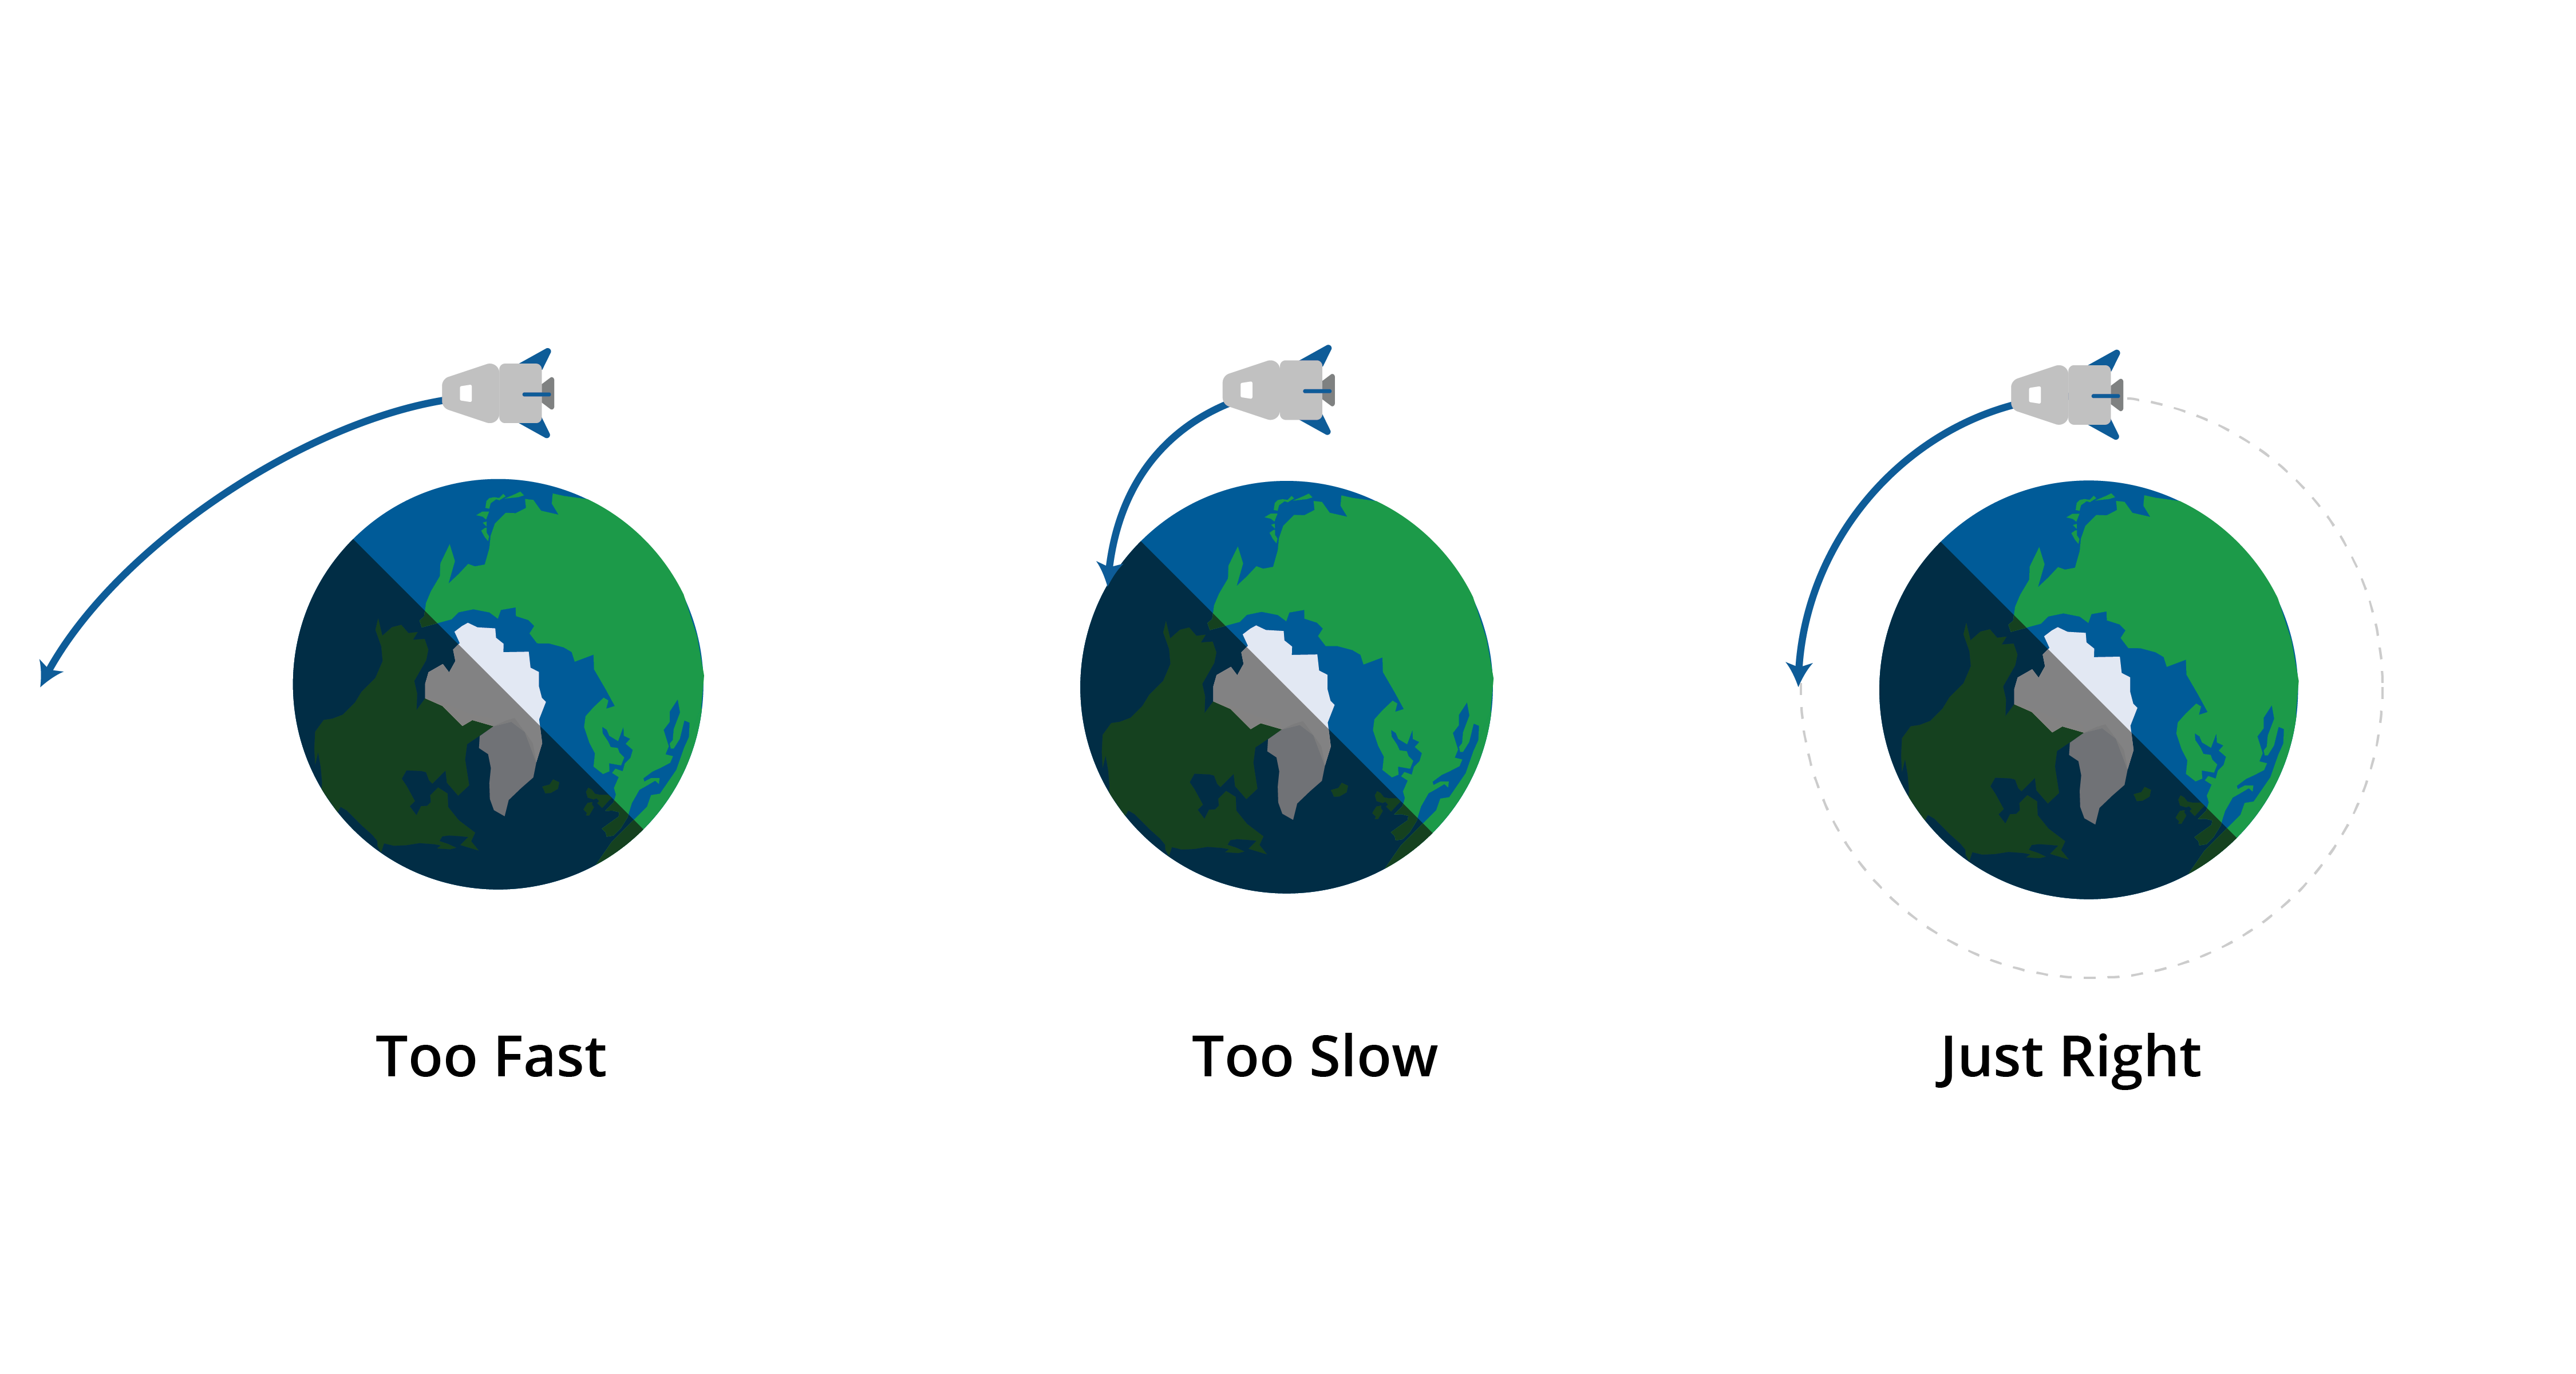
\includegraphics[width=.75\textwidth]{orbitSpeeds.png}
    \caption{A diagram showing the required speeds for entering orbit.}
    \label{fig:orbitSpeeds}
\end{figure}



The radius of the earth is about 6.37 million meters. A satellite that
is in a low orbit is typically about 2 million meters above the
ground. At that distance, the acceleration due to gravity is more like
$6.8 m/s^2$, instead of the $9.8 m/s^2$ that we experience on the
surface of the planet.

How fast does the satellite need to be moving in a circle with a
radius of 8.37 million meters to have an acceleration of $6.8 m/s^2$? Real fast.

Recall that the acceleration vector is

$$a = \frac{v^2}{r}$$

Thus the velocity $v$ needs to be:

$$v = \sqrt{a r} = \sqrt{6.8(8.37 x 10^6)} = 7,544 \text{ m/s}$$

(That's 16,875 miles per hour.)

When a satellite falls out of orbit, it enters the atmosphere at that
7,544 m/s.  The air rushing by generates so much friction that the
satellite gets very, very hot, and usually disintegrates.

\section{Astronauts are \emph{not} weightless}

Some people see astronauts floating inside an orbiting spacecraft and
think there is no gravity: that the astronauts are so far away that
the gravity of the planet doesn't affect them. This is incorrect.  The
gravity might be slightly less (Maybe 6 newtons per kg instead of 9.8
newtons per kg), but the weightless they experience is because they
and the spacecraft is in free fall.  They are just moving so fast (in
a direction perpendicular to gravity) that they don't collide with the
planet.

% 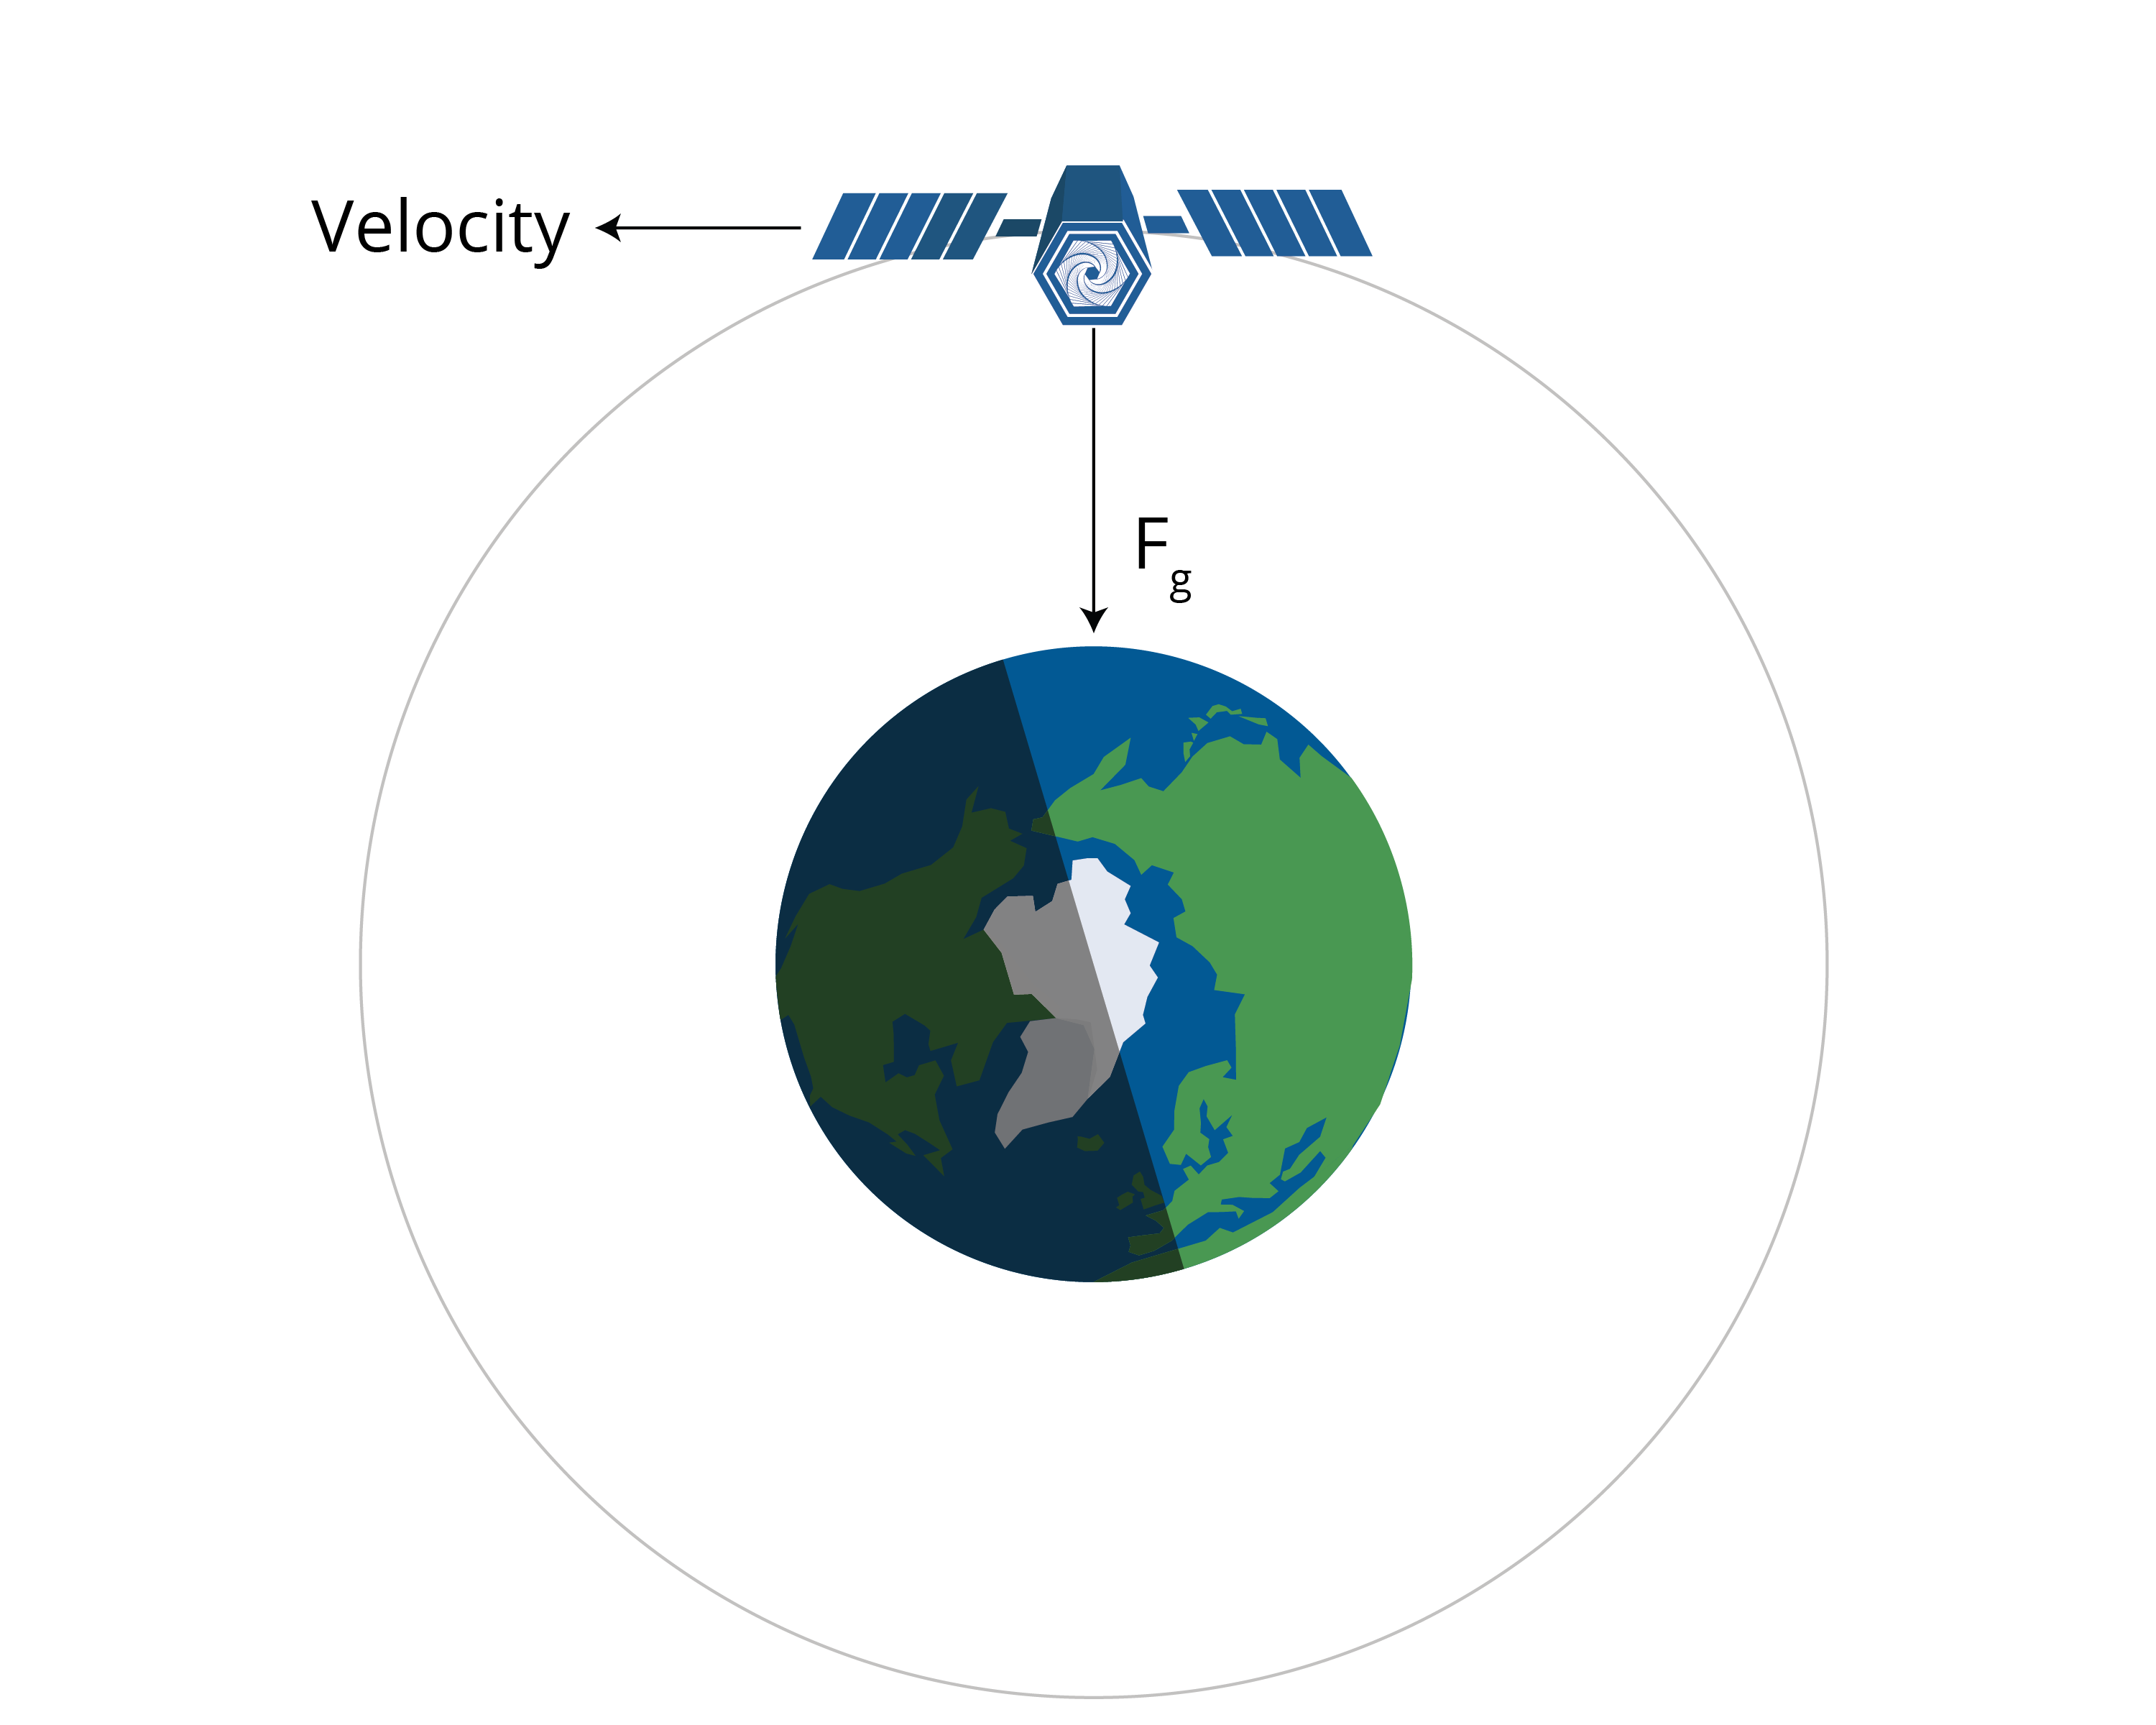
\includegraphics[width=1\textwidth]{satellite.png}


\begin{Exercise}[title={Mars Orbit}, label=mars_orbit]
  
  The radius of Mars is 3.39 million meters. The atmosphere goes up
  another 11 km.  Let's say you want to put a satellite in a circular
  orbit around Mars with a radius of 3.4 million meters.

  The acceleration due to gravity on the surface of Mars is $3.721
  m/s^2$. We can safely assume that it is approximately the same 11 km
  above the surface.

  How fast does the satellite need to be traveling in its orbit?  How
  long will each orbit take?

\end{Exercise}
\begin{Answer}[ref=circular]
  $$v = \sqrt{3.721(3.4 \times 10^6)} = 3,557\text{ m/s}$$

  The circular orbit is $2\pi(3.4 \times 10^6) = 21.4 \times 10^6$ meters in circumference.

  The period of the orbit is $(21.4 \times 10^6)/3,557 \approx 6,000$ seconds.
\end{Answer}

\section{Geosynchronous Orbits}
\index{geosynchronous orbits}
The planet earth rotates once a day.  Satellites in low orbits circle
the earth many times a day. Satellites in very high orbits circle
less than once per day. There is a radius at which a satellite orbits
exactly once per day.  Satellites at this radius are known as
``geosynchronous'' or ``geostationary'', because they are always
directly over a place on the planet.
\begin{figure}[htbp]
    \centering
    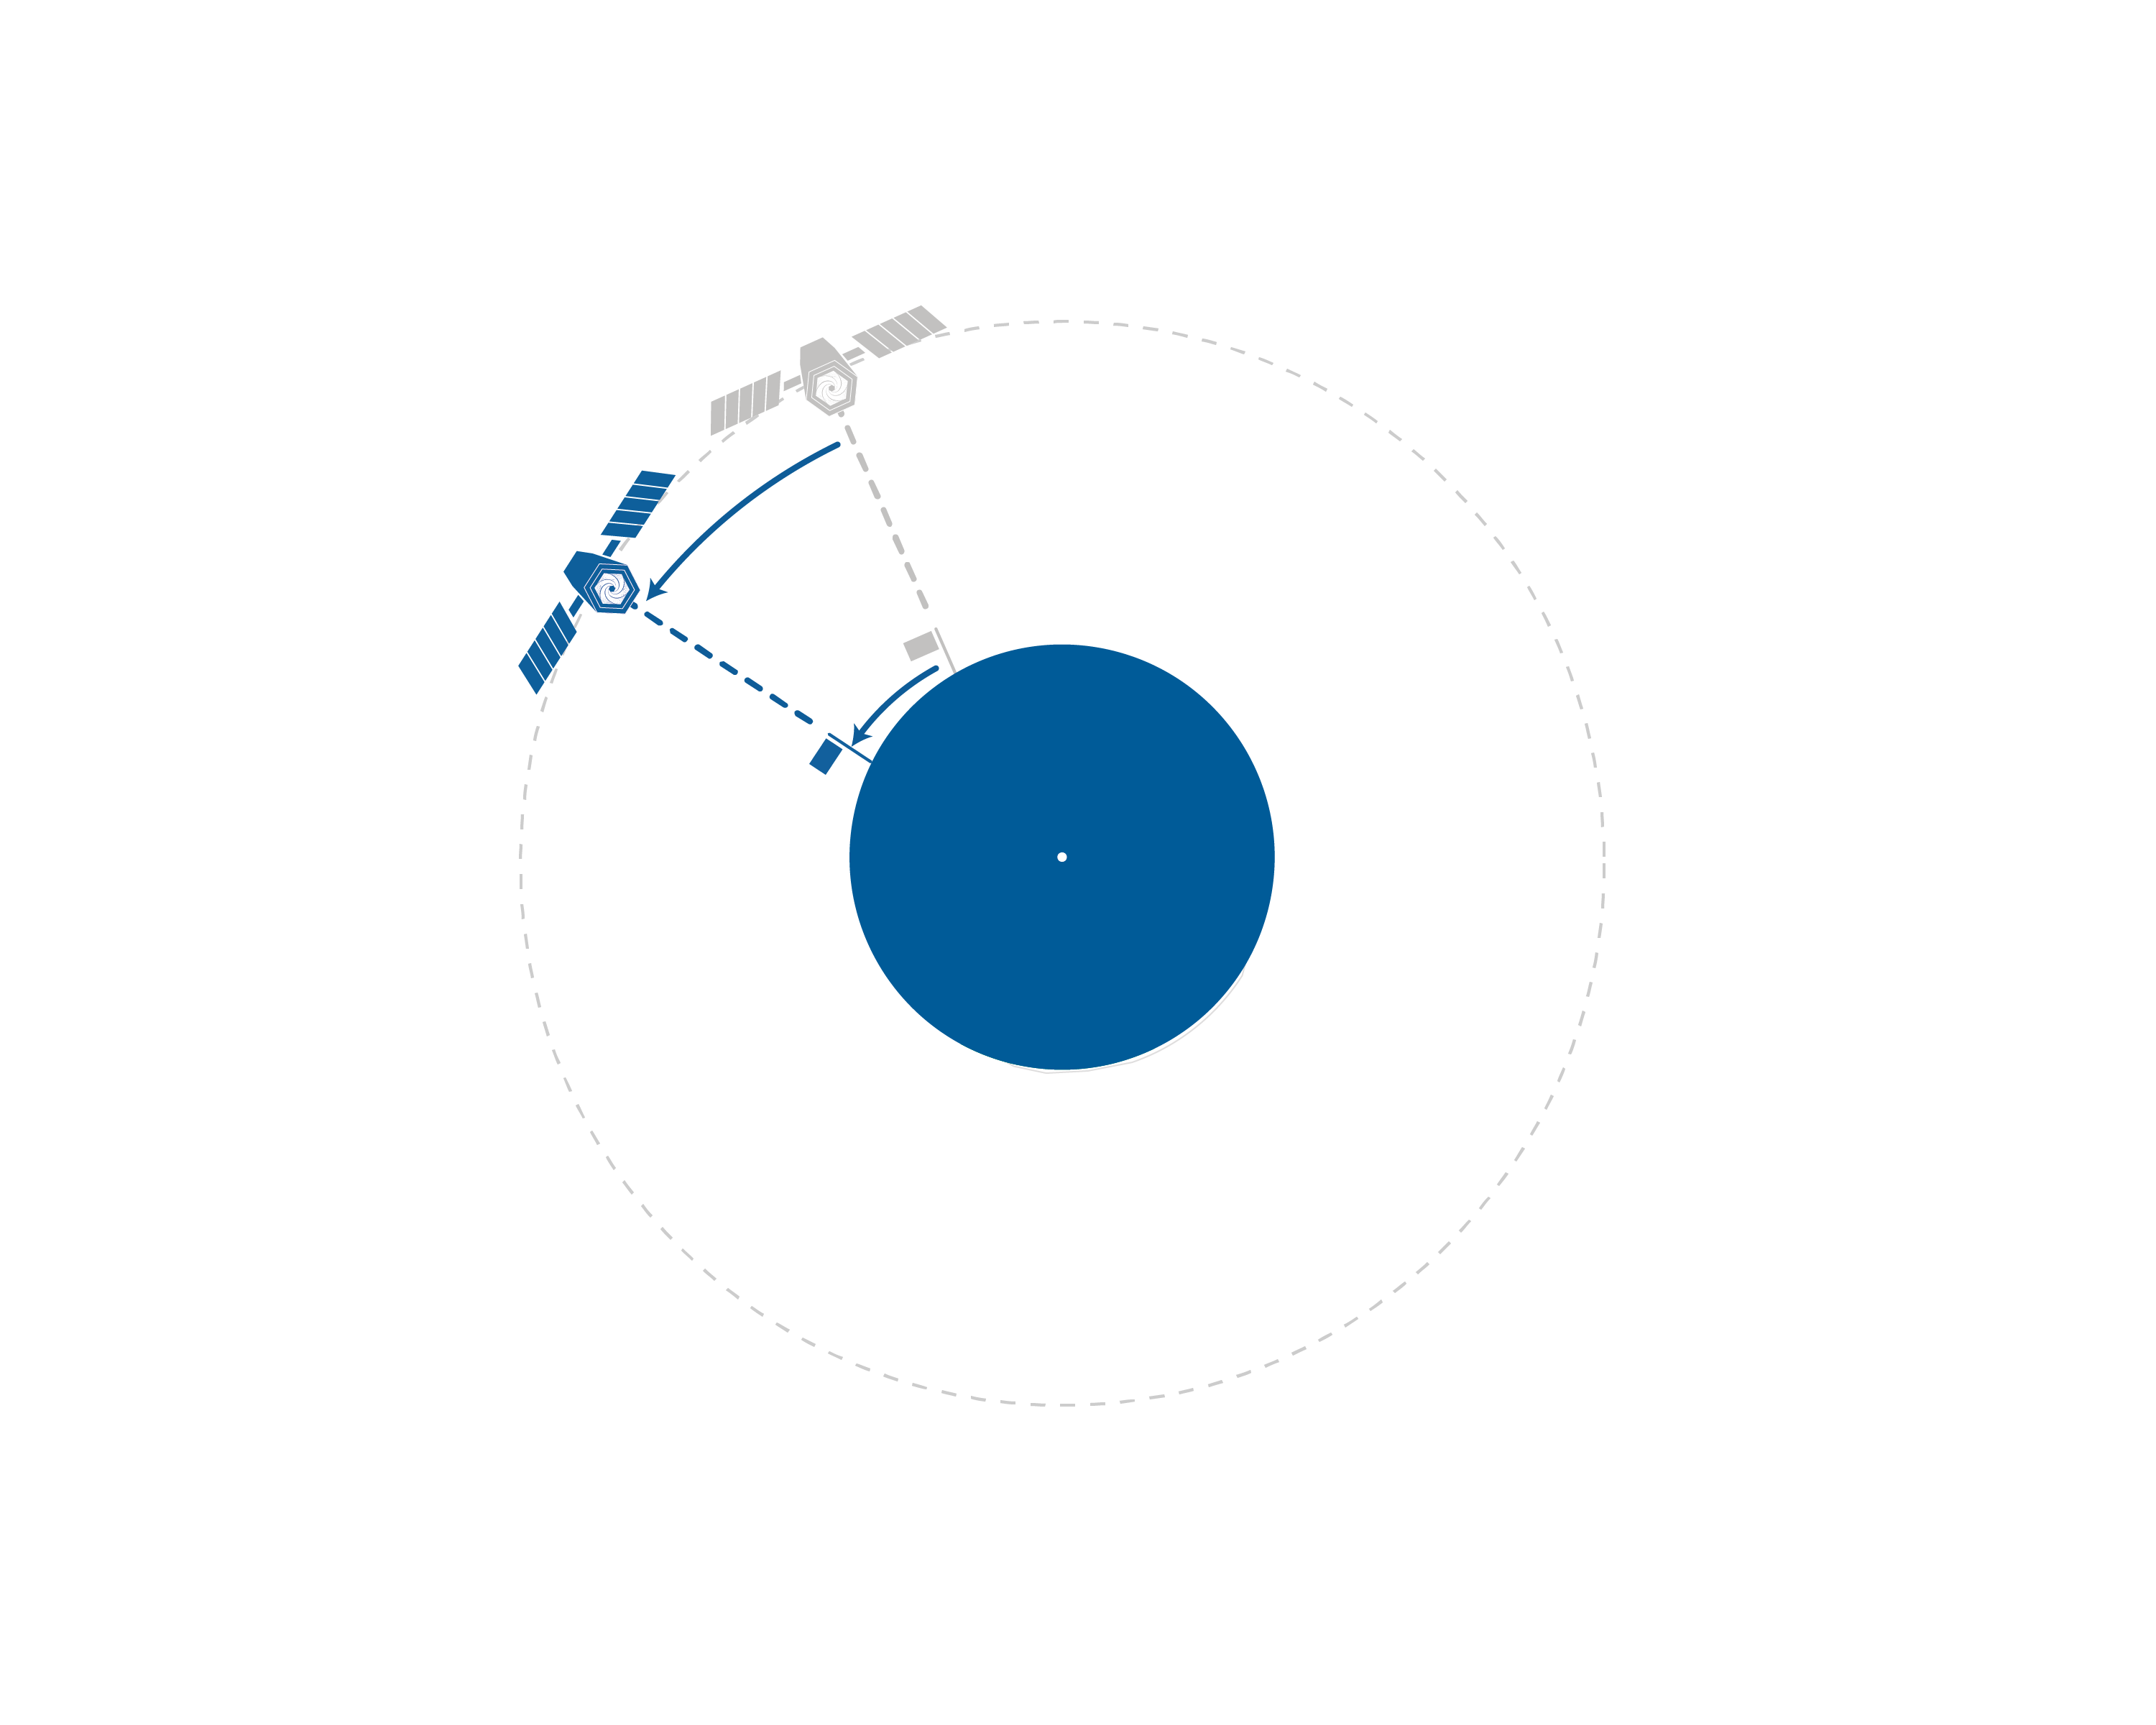
\includegraphics[width=.75\textwidth]{geoSync.png}
    \caption{A satellite in geosynchronous orbit.}
    \label{fig:geoSync}
\end{figure}

The radius of a circular geosynchronous orbit is 42.164 million
meters. (About 36 km above the surface of the earth.)

A geosynchronous satellite travels at a speed of 3,070 m/s.

Geosynchronous satellites are used for the Global Positioning
Satellite system, weather monitoring system, and communications
system.
\section{Escape velocity}
\index{escape velocity}
FIXME: Add text for escape velocity
\begin{figure}[htbp]
    \centering
    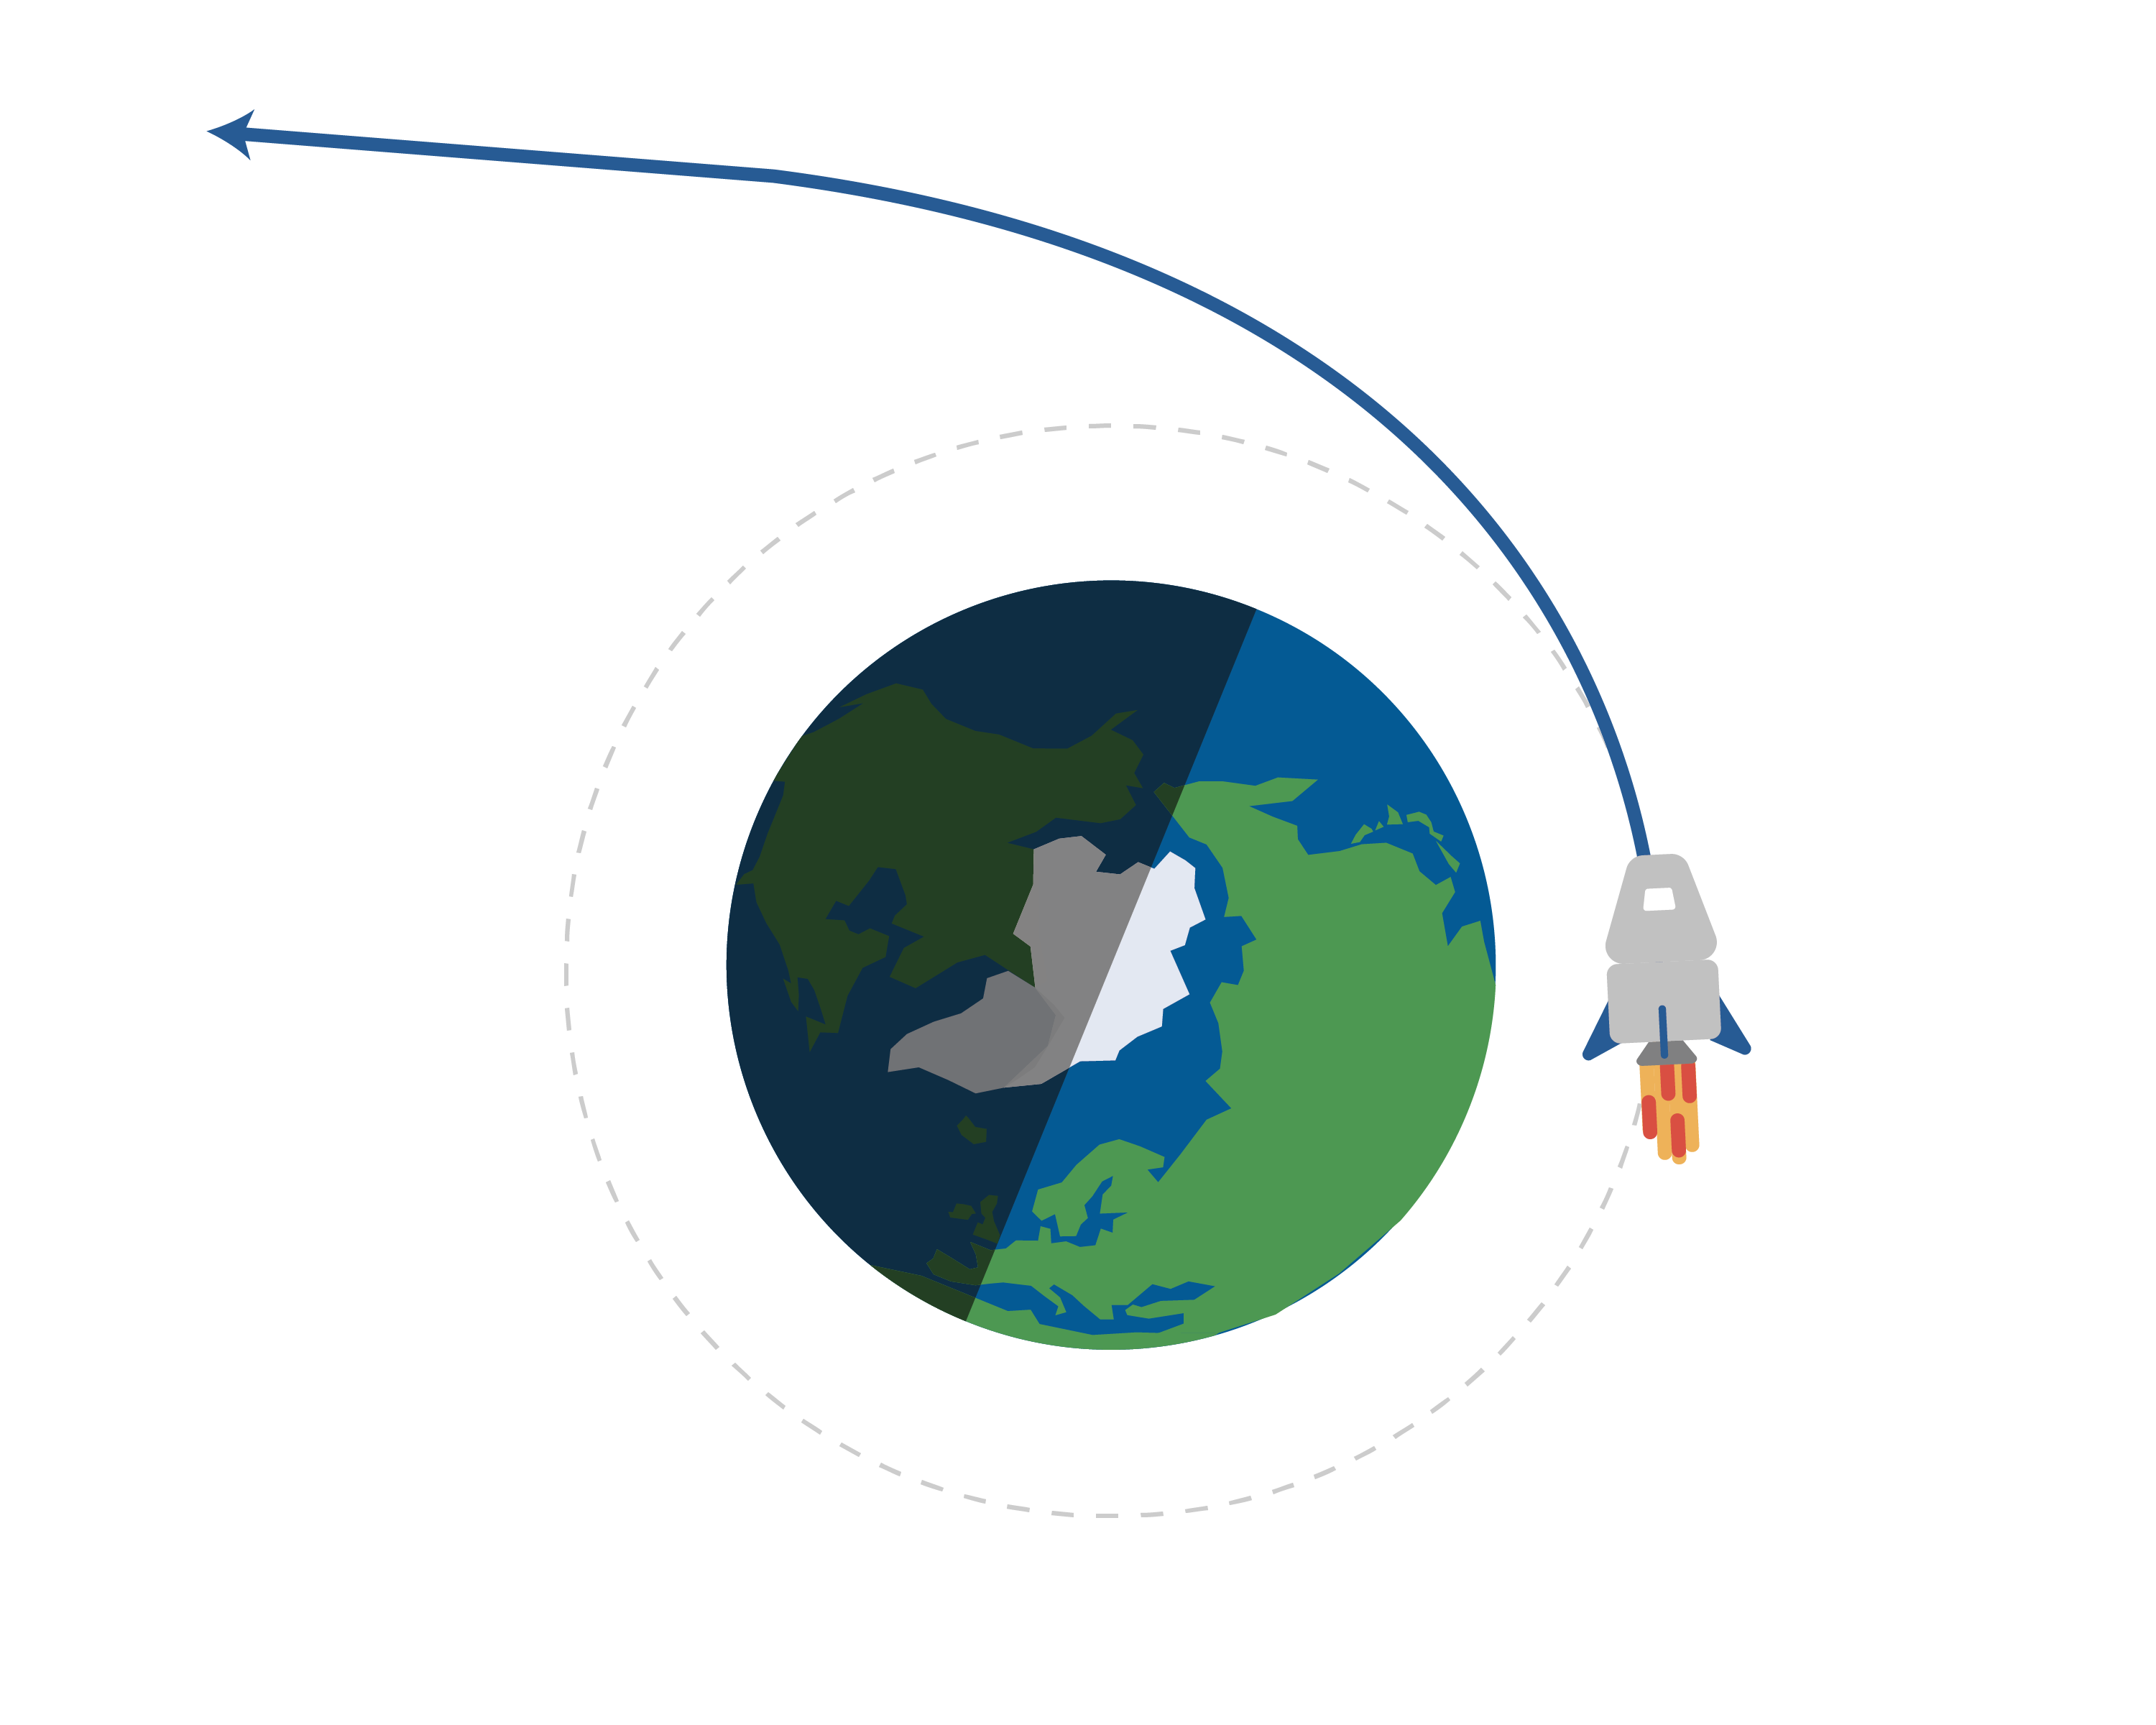
\includegraphics[width=.75\textwidth]{escape.png}
    \caption{A satellite can reach a speed at which it "escapes" earth's orbit (centripetal force).}
    \label{fig:escape}
\end{figure}


%FIXME introduce gravitation (outside of earth gravity) here? Would be good
%%%%%%%%%%%%%%%%%%%%%%%%%%%%%%%%%
%% Bookfooter.tex by Aaron Hillegass
%% Nov 8, 2020

\appendix

\chapter{Answers to Exercises}
\shipoutAnswer

\bibliography{references}

\printindex

\end{document}